% interacttfssample.tex
% v1.05 - August 2017

\documentclass[]{interact}

\usepackage{epstopdf}% To incorporate .eps illustrations using PDFLaTeX, etc.
\usepackage[caption=false]{subfig}% Support for small, `sub' figures and tables
%\usepackage[nolists,tablesfirst]{endfloat}% To `separate' figures and tables from text if required

%\usepackage[doublespacing]{setspace}% To produce a `double spaced' document if required
%\setlength\parindent{24pt}% To increase paragraph indentation when line spacing is doubled
%\setlength\bibindent{2em}% To increase hanging indent in bibliography when line spacing is doubled

\usepackage[numbers,sort&compress]{natbib}% Citation support using natbib.sty
\bibpunct[, ]{[}{]}{,}{n}{,}{,}% Citation support using natbib.sty
\renewcommand\bibfont{\fontsize{10}{12}\selectfont}% Bibliography support using natbib.sty

\theoremstyle{plain}% Theorem-like structures provided by amsthm.sty
\newtheorem{theorem}{Theorem}[section]
\newtheorem{lemma}[theorem]{Lemma}
\newtheorem{corollary}[theorem]{Corollary}
\newtheorem{proposition}[theorem]{Proposition}

\theoremstyle{definition}
\newtheorem{definition}[theorem]{Definition}
\newtheorem{example}[theorem]{Example}

\theoremstyle{remark}
\newtheorem{remark}{Remark}
\newtheorem{notation}{Notation}



















% Other useful packages
\usepackage{bm}

% For fancy look
\usepackage{nicefrac}    % compact symbols for 1/2, etc.
\usepackage{microtype}   % microtypography
\usepackage{booktabs}    % professional-quality tables

% Proper spacing \left \right
\let\originalleft\left
\let\originalright\right
\renewcommand{\left}{\mathopen{}\mathclose\bgroup\originalleft}
\renewcommand{\right}{\aftergroup\egroup\originalright}

% Checkmarks
\usepackage{pifont}% http://ctan.org/pkg/pifont
\newcommand{\cmark}{{\color{mygreen} \ding{51}}}%
\newcommand{\xmark}{{\color{myred} \ding{55}}}

% For creating algorithms
\usepackage[section]{algorithm}
\usepackage{algorithmicx}
\usepackage{algpseudocode}
\renewcommand{\algorithmicrequire}{\textbf{Input:}}
\renewcommand{\algorithmicensure}{\textbf{Output:}}
\algdef{SE}[DOWHILE]{Do}{doWhile}{\algorithmicdo}[1]{\algorithmicwhile\ #1}%


% Some declarations
\newcommand{\norm}[1]{\|#1\|}
\newcommand{\normlr}[1]{\|#1\|}
\newcommand{\nrm}[1]{|#1|}
\newcommand{\nrmlr}[1]{|#1|}
\newcommand{\N}{{\mathbb N}}
\newcommand{\R}{{\mathbb R}}
\newcommand{\EE}{{\mathbb E}}
\newcommand{\PP}{{\mathbb P}}
\newcommand{\bpm}{\begin{pmatrix}}
\newcommand{\epm}{\end{pmatrix}}

\newcommand{\mnmz}{\operatorname*{minimize}}
\newcommand{\mxmz}{\operatorname*{maximize}}
\newcommand{\st}{\operatorname{subject\ to}}
\newcommand{\argmin}{\operatorname*{argmin}}
\newcommand{\eps}{{\varepsilon}}


% And finally some fancy plotting
\usepackage{tikz}
\usepackage{pgfplots}
\usepackage{pgfplotstable}

















%\usepackage[utf8]{inputenc} % allow utf-8 input
%\usepackage[T1]{fontenc}  % use 8-bit T1 fonts
%\usepackage{hyperref}    % hyperlinks
\usepackage{url}      % simple URL typesetting
\usepackage{booktabs}    % professional-quality tables
\usepackage{amsfonts}    % blackboard math symbols
\usepackage{nicefrac}    % compact symbols for 1/2, etc.
\usepackage{microtype}   % microtypography

\usepackage{xspace}
\usepackage{enumitem}


\usepackage{comment}
\usepackage{array}
\usepackage{units}
\usepackage{bm}
\usepackage{amsmath}
\usepackage{amssymb}
\usepackage{graphicx}
\usepackage[section]{algorithm}
\usepackage{algorithmicx}
\usepackage{algpseudocode}
\renewcommand{\algorithmicrequire}{\textbf{Input:}}
\renewcommand{\algorithmicensure}{\textbf{Output:}}








% Added by lyx2lyx
\renewcommand{\textendash}{--}
\renewcommand{\textemdash}{---}




%added by Pevnak
\usepackage{color}
\newcommand{\tpnote}[1]{{\color{magenta}#1}}

%tracking changes
\usepackage{todonotes}
\usepackage[normalem]{ulem}

\newcommand{\sdot}[0]{\mkern1mu{\cdot}\mkern1mu}





\newcommand{\atoppush}{TopPush\xspace}
\newcommand{\atoppushk}{TopPushK\xspace}
\newcommand{\agrill}{Grill\xspace}
\newcommand{\apatmat}{Pat\&Mat\xspace}
\newcommand{\atopmeank}{TopMean\xspace}
\newcommand{\anpA}{Grill-NP\xspace}
\newcommand{\anpB}{Pat\&Mat-NP\xspace}
\newcommand{\anpC}{$\tau$-FPL\xspace}

\newcommand{\toppush}{\emph{TopPush}\xspace}
\newcommand{\toppushk}{\emph{TopPushK}\xspace}
\newcommand{\grill}{\emph{Grill}\xspace}
\newcommand{\patmat}{\emph{Pat}\&\emph{Mat}\xspace}
\newcommand{\topmeank}{\emph{TopMean}\xspace}
\newcommand{\npA}{\emph{Grill-NP}\xspace}
\newcommand{\npB}{{\emph{Pat}\&\emph{Mat-NP}}\xspace}
\newcommand{\npC}{{\emph{$\tau$-FPL}}\xspace}

\newcommand{\TopPush}{\emph{TopPush}\xspace}
\newcommand{\TopPushK}{\emph{TopPushK}\xspace}
\newcommand{\TopMean}{\emph{TopMean}\xspace}
\newcommand{\PatMat}{\emph{Pat}\&\emph{Mat}\xspace}
\newcommand{\PatMatNP}{{\emph{Pat}\&\emph{Mat-NP}}\xspace}
\newcommand{\Grill}{\emph{Grill}\xspace}
\newcommand{\GrillNP}{\emph{Grill-NP}\xspace}
\newcommand{\tauFPL}{{\emph{$\tau$-FPL}}\xspace}


\newcommand{\tp}{\textnormal{tp}}
\newcommand{\tn}{\textnormal{tn}}
\newcommand{\fp}{\textnormal{fp}}
\newcommand{\fn}{\textnormal{fn}}
\newcommand{\tps}{\overline{\textnormal{tp}}}
\newcommand{\tns}{\overline{\textnormal{tn}}}
\newcommand{\fps}{\overline{\textnormal{fp}}}
\newcommand{\fns}{\overline{\textnormal{fn}}}

\newcommand{\Xcal}{\mathcal{X}}


















\usepackage{colortbl}
\colorlet{tableheadcolor}{gray!25} % Table header colour = 25% gray
\newcommand{\headcol}{\rowcolor{tableheadcolor}}            





\usepackage{graphics}
\usepackage{xcolor}
\definecolor{myred}{RGB}{204, 0, 0}
\definecolor{mygreen}{RGB}{0, 153, 0}
\definecolor{myblue}{RGB}{0, 153, 255}
\definecolor{myorange}{RGB}{255, 153, 51}








% And finally some fancy plotting
\usepackage{pgfplots}
\usepackage{pgfplotstable}
\usetikzlibrary{pgfplots.groupplots}
\pgfplotsset{compat=1.3}
\pgfplotsset{
    line1/.style={%
        myred, thick},
    line2/.style={%
        myblue, thick, dashed},
    line3/.style={%
        mygreen, thick, dotted},
    line4/.style={%
        myorange, thick, dashdotted},
    col1/.style={%
        xmin=0, xmax=1,
        xtick={0,0.2,0.4,0.6,0.8}},
    col2/.style={%
        xmin=0, xmax=0.1,
        xtick={0,0.02,0.04,0.06,0.08},
        xticklabels={0,0.02,0.04,0.06,0.08}},
    col3/.style={%
        xmin=0, xmax=0.01,
        xtick={0,0.002,0.004,0.006,0.008},
        xticklabels={0,0.002,0.004,0.006,0.008},
        scaled x ticks=false},
    legendStyleA/.style={%
        column sep = 10pt,
        legend columns = -1,
        legend to name = grouplegendA},
}


\usepackage{pgfplotstable}
\usetikzlibrary{pgfplots.groupplots}


\definecolor{myred}{RGB}{204, 0, 0}
\definecolor{mygreen}{RGB}{0, 153, 0}
\definecolor{myblue}{RGB}{0, 153, 255}
\definecolor{myorange}{RGB}{255, 153, 51}

\pgfplotsset{
    LinePatMatNP/.style={mygreen, very thick},
    LineTopPush/.style={myred, very thick, dashed},
    LinePatMat/.style={myblue, very thick, dotted},
    LinetauFPL/.style={myorange, very thick, dashdotted},
}

\pgfplotstableread[col sep = comma]{data/CIFAR100.csv}\DataCIFAR
\pgfplotstableread[col sep = comma]{data/HEPMASS.csv}\DataHEPMASS










\newcommand{\theoremNN}[2]{\noindent\textbf{Theorem \ref{#1} (page \pageref{#1})}\ \emph{#2}}
\newcommand{\propositionNN}[2]{\noindent\textbf{Proposition \ref{#1} (page \pageref{#1})}\ \emph{#2}}






\usepackage{a4wide}


\newcommand{\NEW}[1]{{\color{blue} #1}}


\begin{document}

\articletype{}% Specify the article type or omit as appropriate

\title{General Framework for Binary Classification on Top Samples}

\author{
\name{L. Adam\textsuperscript{a}\thanks{Email: lukas.adam.cr@gmail.com}, V. M\'acha\textsuperscript{b}, V. \v{S}m\'idl\textsuperscript{a,c} and T. Pevn\'y\textsuperscript{a}}
\affil{\textsuperscript{a} Faculty of Electrical Engineering, Czech Technical University in Prague, Prague, Czech Republic \\
\textsuperscript{b} Faculty of Nuclear Sciences and Physical Engineering, Czech Technical University in Prague, Prague, Czech Republic \\ 
\textsuperscript{c}The Czech Academy of Sciences, Institute of Information Theory and Automation, Pod Vod\'arenskou v{\v ez}\'i 4, 182 08 Prague, Czech Republic.}
}

\maketitle

\begin{abstract}
Many binary classification problems minimize misclassification above (or below) a threshold. We show that instances of ranking problems, accuracy at the top, or hypothesis testing may be written in this form. We propose a general framework to handle these classes of problems and show which formulations (both known and newly proposed) fall into this framework. We provide a theoretical analysis of this framework and mention selected possible pitfalls the formulations may encounter. We show the convergence of the stochastic gradient descent for selected formulations even though the gradient estimate is inherently biased. We suggest several numerical improvements, including the implicit derivative and stochastic gradient descent. We provide an extensive numerical study. %Based both on the theoretical properties and numerical experiments, we conclude the paper by suggesting which method should be used in which situation.
\end{abstract}

\begin{keywords}
General framework; Classification; Ranking; Accuracy at the Top; Neyman-Pearson; Pat\&Mat.
\end{keywords}

\begin{amscode}
90C20; 49M05; 65K10; 49K10.
\end{amscode}










\section{Introduction}\label{sec:Motivation}



Many binary classification problems focus on separating the dataset by a linear hyperplane $\bm w^\top \bm x-t$. A sample $\bm x$ is deemed to be positive or relevant (depending on the application) if its score $\bm w^\top \bm x$ is above a threshold $t$. Multiple problem categories belong to this framework:
\begin{itemize}\itemsep 0pt
%\item \textit{Support vector machines} where the threshold equals the offset of the separating hyperplane. The accuracy is evaluated for the whole dataset.
\item \textit{Ranking problems} select the most relevant samples and rank them. To each sample, a numerical score is assigned, and the ranking is performed based on this score. Often, only scores above a threshold are considered.
\item \textit{Accuracy at the Top} is similar to ranking problems. However, instead of ranking the most relevant samples, it only maximizes the accuracy (equivalently minimizes the misclassification) in these top samples. The prime examples of both categories include search engines or problems where identified samples undergo expensive post-processing such as human evaluation.
\item \textit{Hypothesis testing} states a null and an alternative hypothesis. The Neyman-Pearson problem minimizes the Type II error (the null hypothesis is false but it fails to be rejected) while keeping the Type I error (the null hypothesis is true but is rejected) small. If the null hypothesis states that a sample has the positive label, then Type II error happens when a positive sample is below the threshold and thus minimizing the Type II error amounts to minimizing the positives below the threshold.
\end{itemize}
\NEW{Examples of this type can be found in search engines, where the user is interested only in the first few queries. These queries need to be of high quality. Other examples include cybersecurity~\cite{Grill_2016}, where a low false-negative rate is crucial as a high number of false alarms would result in the software being uninstalled, or drug development, where potentially useful drugs need to be preselected and manually investigated.} All these three applications may be written (possibly after a reformulation) in a similar form as a minimization of the false-negatives (misclassified positives) above a threshold. They only differ in the way they define the threshold. Despite this striking similarity, they are usually considered separately in the literature. The main goal of this paper is to provide a unified framework for these three applications and perform its theoretical and numerical analysis.

The goal of the ranking problems is to rank the relevant samples higher than the non-relevant ones. A prototypical example is the RankBoost \citep{freund2003efficient} maximizing the area under the ROC curve, the Infinite Push \citep{agarwal2011infinite} or the $p$-norm push \citep{rudin.2009} which concentrate on the high-ranked negatives and push them down. Since all these papers include pairwise comparisons of all samples, they can be used only for small datasets. This was alleviated in \cite{Li_TopPush}, where the authors performed the limit $p\to\infty$ in $p$-norm push and obtained the linear complexity in the number of samples. Moreover, since the $l_{\infty}$-norm is equal to the maximum, this method falls into our framework with the threshold equal to the largest score computed from negative samples.

Accuracy at the Top ($\tau$-quantile) was formally defined in \cite{boyd2012accuracy} and maximizes the number of relevant samples in the top $\tau$-fraction of ranked samples. When the threshold equals the top $\tau$-quantile of all scores, this problem falls into our framework. The early approaches aim at solving approximations, for example, \cite{Joachims:2005:SVM:1102351.1102399} optimizes a convex upper bound on the number of errors among the top samples. Due to the presence of exponentially many constraints, the method is computationally expensive. \cite{boyd2012accuracy} presented an SVM-like formulation which fixes the index of the quantile and solves $n$ problems. While this removes the necessity to handle the (difficult) quantile constraint, the algorithm is computationally infeasible for a large number of samples. \cite{kar2015surrogate} derived upper approximations, their error bounds and solved these approximations. \cite{Grill_2016} proposed the projected gradient descent method where after each gradient step, the quantile is recomputed. \cite{Eban_2017} suggested new formulations for various criteria and argued that they keep desired properties such as convexity. %\cite{mackey2018constrained} generalized this paper by considering a more general setting.
\cite{tasche2018plug} showed that accuracy at the top is maximized by thresholding the posterior probability of the relevant class. The closest approach to our framework is \cite{lapin.2015,lapin2018analysis}, where the authors considered multi-class classification problems, and their goal was to optimize the performance on the top few classes and \cite{mackey2018constrained}, where the authors implicitly removed some variables and derived an efficient algorithm.

The paper is organized as follows. In Section \ref{sec:framework}, we introduce the unified framework and then show how the three applications above fall into it. To each application, we state several numerical formulations, some of them are known, and some are new. In Section \ref{sec:theory}, we perform a theoretical analysis of the unified framework. First, we focus on convexity, which ensures that no local minima are present. Second, we show which formulations from the previous section are differentiable. Finally, we present a simple example which shows the differences between these formulations and highlights the major problem that some of the formulations may have a global minimum at $\bm w=0$. Since the weights form the normal of the separating hyperplane, this solution does not provide any information. We further build on this example and analyze the case when zero weights are the global minimum. We show that the higher the threshold, the more likely a problem is to have the global minimum at zero. Based on this result, we compare the thresholds of individual formulations and show how stable they are. Section \ref{sec:convergence} argues that the threshold $t$ depends on the weights $\bm w$ and therefore, we follow the implicit programming technique and remove the threshold constraint. We show how to compute derivatives for the reduced problem. We propose a more complex stochastic gradient descent method which is convergent. Section \ref{sec:num1} presents the numerical results. We show both a good performance of our method and verify the theoretical results numerically. To keep the brevity of the paper, we postpone multiple results to the Appendix. The reader is welcome to refer to our codes online.\footnote{\texttt{https://github.com/VaclavMacha/AccuracyAtTopPrimal\_experiments.jl}}

%The paper is concluded by a recommendation stating which methods should be used in which situations. This recommendation is based both on theoretical and numerical analysis. 




\section{Framework for Minimizing Missclassification Above a Threshold}\label{sec:framework}

Many important binary classification problems minimize the number of misclassified samples below (or above) certain threshold. Since these problems are usually considered separately, in this section, we provide a unified framework for their handling and present several classification problems falling into this framework.

For samples $\bm x$, we consider the linear classifier $f(\bm w)=\bm w^\top \bm x-t$, where $\bm w$ is the normal vector to the separating hyperplane and $t$ is a threshold. The most well-known example is the support vector machines, where $t$ is an optimization variable. In many cases the threshold $t$ is computed from the scores $z=\bm w^\top \bm x$. For example, \toppush from \cite{Li_TopPush} sets the threshold $t$ to the largest score $z^-$ corresponding to negative samples and \cite{Grill_2016} sets it to the quantile of all scores.

To be able to determine the missclassification above and below the threshold $t$, we define the true-positive, false-negative, true-negative and false-positive counts by
\begin{equation}\label{eq:defin_counts}
\aligned
\tp(\bm w,t) & = \sum_{\bm x\in\mathcal X^+}\left[\bm w^\top \bm x-t \ge 0\right], &
\fn(\bm w,t) & = \sum_{\bm x\in\mathcal X^+}\left[\bm w^\top \bm x-t < 0\right], \\
\tn(\bm w,t) & = \sum_{\bm x\in\mathcal X^-}\left[\bm w^\top \bm x-t < 0\right], &
\fp(\bm w,t) & = \sum_{\bm x\in\mathcal X^-}\left[\bm w^\top \bm x-t \ge 0\right].
\endaligned
\end{equation}
Here $[\cdot]$ is the 0-1 loss (Iverson bracket, characteristic function) which is equal to $1$ if the argument is true and to $0$ otherwise. Moreover, $\mathcal{X}/\mathcal{X}^{+}/\mathcal{X}^{-}$ denotes the sets of all/positive/negative samples and by $n/n^{+}/n^{-}$ their respective sizes. 

Since the misclassified samples below the threshold are the false-negatives, we arrive at the following problem
\begin{equation}\label{eq:problem1}
\aligned
{\rm minimize} & \quad\frac{1}{n^{+}}\fn(\bm w,t)\\
\textnormal{subject to} & \quad \text{threshold }t\text{ is a function of }\{\bm w^\top \bm x_i\}_{i=1}^n.
\endaligned
\end{equation}
As the 0-1 loss in \eqref{eq:defin_counts} is discontinuous, problem \eqref{eq:problem1} is difficult to handle. The usual approach is to employ a surrogate function such as the hinge loss function defined by
\begin{equation}\label{eq:defin_surrogate}
\aligned
l_{\rm hinge}\left(z\right) & =\max\left\{ 0,1+z\right\}. \\
%l_{\log}\left(z\right) & =\frac{1}{\log2}\log\left(1+e^z\right).
\endaligned
\end{equation}
In the text below, the symbol $l$ denotes any convex non-negative non-decreasing function with $l(0)=1$. Using the surrogate function, the counts \eqref{eq:defin_counts} may be approximated by their surrogate counterparts
\begin{equation}\label{eq:defin_counts_surr}
\aligned
\tps(\bm w ,t) & = \sum_{\bm x\in\mathcal{X}^+}l(\bm w^\top \bm x-t), &
\fns(\bm w ,t) & = \sum_{\bm x\in\mathcal{X}^+}l(t-\bm w^\top \bm x), \\
\tns(\bm w ,t) & = \sum_{\bm x\in\mathcal{X}^-}l(t-\bm w^\top \bm x),&
\fps(\bm w ,t) & = \sum_{\bm x\in\mathcal{X}^-}l(\bm w^\top \bm x-t).
\endaligned
\end{equation}
Since $l(\cdot)\ge[\cdot]$, the surrogate counts \eqref{eq:defin_counts_surr} provide upper approximations of the true counts \eqref{eq:defin_counts}. Replacing the counts in \eqref{eq:problem1} by their surrogate counterparts and adding a regularization results in
\begin{equation}\label{eq:problem2}
\aligned
{\rm minimize} & \quad\frac{1}{n^{+}}\fns(\bm w,t) + \frac\lambda2\norm{\bm w}^2 \\
\textnormal{subject to} & \quad \text{threshold }t\text{ is a function of }\{\bm w^\top \bm x_i\}_{i=1}^n.
\endaligned
\end{equation}
In the rest of this section, we list formulations which fall into the framework of \eqref{eq:problem1} and \eqref{eq:problem2}.


\subsection{Methods based on pushing positives to the top}\label{sec:obj1}

The first category of formulations falling into our framework \eqref{eq:problem1} and \eqref{eq:problem2} are ranking methods which attempt to put as many positives (relevant samples) to the top as possible. Specifically, for each sample $\bm x$, they compute the score $z=\bm w^\top \bm x$ and then sort the vector $\bm z$ into $\bm z_{[\cdot]}$ with decreasing components $z_{[1]}\ge z_{[2]}\ge\dots\ge z_{[n]}$. The number of positives on top equals to the number of positives above the highest negative. This amounts to maximizing true-positives or, equivalently, minimizing false-negatives, which may be written as
\begin{equation}\label{eq:problem_top2}
\aligned
{\rm minimize} & \quad\frac{1}{n^{+}}\fn(\bm w,t) \\
\textnormal{subject to} & \quad t = z_{[1]}^-, \\
& \quad \text{components of }\bm z^-\text{ equal to }z^-=\bm w^\top \bm x^-\text{ for }\bm x^- \in \Xcal^-.
\endaligned
\end{equation}
As $t$ is a function of the scores $z=\bm w^\top \bm x$, problem \eqref{eq:problem_top2} is a special case of \eqref{eq:problem1}.


\toppush from \citep{Li_TopPush} replaces the false-negatives in \eqref{eq:problem_top2} by their surrogate and adds a regularization term to arrive at
\begin{equation}\label{eq:problem_toppush}
\aligned
{\rm minimize} & \quad\frac{1}{n^{+}}\fns(\bm w,t) + \frac\lambda2\norm{\bm w}^2 \\
\textnormal{subject to} & \quad t = z_{[1]}^-, \\
& \quad \text{components of }\bm z^-\text{ equal to }z^-=\bm w^\top \bm x^-\text{ for }\bm x^- \in \Xcal^-.
\endaligned
\end{equation}
Note that this falls into the framework of \eqref{eq:problem2}.

As we will show in Section \ref{sec:stability}, \toppush is sensitive to outliers and mislabelled data. To robustify it, we follow the idea from \cite{lapin.2015} and propose to replace the largest negative score by the mean of $k$ largest negative scores. This results in
\begin{equation}\label{eq:problem_toppushk}
\aligned
{\rm minimize} & \quad\frac{1}{n^{+}}\fns(\bm w,t) + \frac\lambda2\norm{\bm w}^2 \\
\textnormal{subject to} & \quad t = \frac 1k(z_{[1]}^- + \dots + z_{[k]}^-), \\
& \quad \text{components of }\bm z^-\text{ equal to }z^-=\bm w^\top \bm x^-\text{ for }\bm x^- \in \Xcal^-.
\endaligned
\end{equation}
We used the mean of highest $k$ negative scores instead of the value of the $k$-th negative score to preserve convexity as shown in Section \ref{sec:convexity}.


\subsection{Accuracy at the Top}\label{sec:obj2}

The previous category considers formulations which minimize the false-negatives below the highest-ranked negative. Accuracy at the Top \citep{boyd2012accuracy} takes a different approach and minimizes false-positives above the top $\tau$-quantile defined by
\begin{equation}\label{eq:defin_quantile} 
t_1(\bm w) = \max\left\{t\mid \tp(\bm w,t) + \fp(\bm w,t)\ge n\tau\right\}.
\end{equation}
Then the Accuracy at the Top problem is defined by
\begin{equation}\label{eq:problem_aatp_orig}
\aligned
{\rm minimize} & \quad \frac{1}{n^{-}}\fp(\bm w,t) \\
\textnormal{subject to} & \quad t\text{ is the top \ensuremath{\tau}-quantile: it solves }\eqref{eq:defin_quantile}.
\endaligned
\end{equation}
Due to Lemma \ref{lemma:fnfp_equivalence} in the Appendix, the previous problem \eqref{eq:problem_aatp_orig} is equivalent (up to a small theoretical issue) to
\begin{equation}\label{eq:problem_aatp}
\aligned
{\rm minimize} & \quad \mu\fn(\bm w,t) + (1-\mu)\fp(\bm w,t) + \frac{\lambda}{2}\norm{\bm w}^2\\
\textnormal{subject to} & \quad t\text{ is the top \ensuremath{\tau}-quantile: it solves }\eqref{eq:defin_quantile}
\endaligned
\end{equation}
for any $\mu\in[0,1]$. This problem with $\mu=0$ equals to \eqref{eq:problem_aatp_orig}, with $\mu=1$ it falls into our framework \eqref{eq:problem1}, while with $\mu=\frac{n^-}{n}$ it corresponds to the original definition from \cite{boyd2012accuracy}. 

Apart from the quantile \eqref{eq:defin_quantile}, there are two other possible choices of the threshold
\begin{align}
\label{eq:defin_quantile1}t_2(\bm w) =\ &\frac{1}{n\tau}\sum_{i=1}^{n\tau} z_{[i]}, \\
\label{eq:defin_quantile0} t_3(\bm w)\quad \text{solves} \quad &\frac1n\sum_{i=1}^nl(\beta(z_i-t)) = \tau.
\end{align}
We again use the vector of scores $\bm z$ with components $z_i=\bm w^\top \bm x_i$ and for the rest of the paper we assume, for simplicity, that $n\tau$ is an integer. The quantile \eqref{eq:defin_quantile} is sometimes denoted as VaR (value at risk) and \eqref{eq:defin_quantile1} as CVaR (conditional value of risk). It is known is that the latter is the tightest convex approximation of the former. We will sometimes denote \eqref{eq:defin_quantile0} as surrogate top $\tau$-quantile. We will investigate the relations between these three objects as well as their properties such as convexity, differentiability or stability in Section \ref{sec:theory}.

Paper \cite{Grill_2016} builds on the Accuracy at the Top problem~\eqref{eq:problem_aatp}, where it replaces $\fn(\bm w, t)$ and $\fp(\bm w, t)$ in the objective by their surrogate counterparts $\fns(\bm w, t)$ and $\fps(\bm w, t)$. This leads to
\begin{equation}\label{eq:problem_grill}
\aligned
{\rm minimize} & \quad \frac{1}{n^{+}}\fns(\bm w,t) + \frac{1}{n^{-}}\fps(\bm w,t) + \frac\lambda2\norm{\bm w}^2\\
\textnormal{subject to} & \quad t\text{ is the top \ensuremath{\tau}-quantile: it solves }\eqref{eq:defin_quantile}.
\endaligned
\end{equation}
Based on the first author, we name this formulation \grill. The main purpose of \eqref{eq:defin_quantile1} is to provide a convex approximation of the non-convex quantile \eqref{eq:defin_quantile}. Putting it into the constraint results in a convex approximation problem, which we call \topmeank
\begin{equation}\label{eq:problem_topmeank}
\aligned
{\rm minimize} & \quad\frac{1}{n^{+}}\fns(\bm w,t) + \frac\lambda2\norm{\bm w}^2 \\
\textnormal{subject to} & \quad t = \frac 1{n\tau}(z_{[1]} + \dots + z_{[n\tau]}), \\
& \quad \text{components of }\bm z\text{ equal to }z=\bm w^\top \bm x\text{ for }\bm x \in \Xcal.
\endaligned
\end{equation}
Similarly, we can use the surrogate top quantile in the constraint to arrive at
\begin{equation}\label{eq:problem_patmat}
\aligned
{\rm minimize} & \quad \frac{1}{n^{+}}\fns(\bm w,t) + \frac\lambda2\norm{\bm w}^2\\
\textnormal{subject to} & \quad t\text{ is the surrogate top \ensuremath{\tau}-quantile: it solves }\eqref{eq:defin_quantile0}.
\endaligned
\end{equation}
Note that \grill minimizes the convex combination of false-positives and false-negatives while~\eqref{eq:problem_topmeank} and \eqref{eq:problem_patmat} minimize only the false-negatives. The reason for this will be evident in Section \ref{sec:convexity} and amounts to preservation of convexity. Moreover, as will see later, problem \eqref{eq:problem_patmat} provides a good approximation to the Accuracy at the Top problem, it is easily solvable due to convexity and requires almost no tuning, we named it \patmat{} (Precision At the Top \& Mostly Automated Tuning). 


\subsection{Methods optimizing the Neyman-Pearson criterion}\label{sec:obj3}

Another category falling into the framework of \eqref{eq:problem1} and \eqref{eq:problem2} is the Neyman-Pearson problem which is closely related to hypothesis testing, where null $H_0$ and alternative $H_1$ hypotheses are given. Type~I error occurs when $H_0$ is true but is rejected, and type II error happens when $H_0$ is false, but it fails to be rejected. The standard technique is to minimize Type II error while a bound for Type I error is given.

In the Neyman-Pearson problem, the null hypothesis $H_0$ states that a sample $\bm x$ has the negative label. Then Type I error corresponds to false-positives while Type II error to false-negatives. If the bound on Type I error equals $\tau$, we may write this as
\begin{equation}\label{eq:defin_quantile_np} 
t_1^{\rm NP}(\bm w) = \max\left\{t\mid \fp(\bm w,t)\ge n^-\tau\right\}.
\end{equation}
Then, we may write the Neyman-Pearson problem as
\begin{equation}\label{eq:problem_np}
\aligned
{\rm minimize} & \quad \frac{1}{n^{+}}\fn(\bm w,t) \\
\textnormal{subject to} & \quad t\text{ is Type I error at level \ensuremath{\tau}: it solves }\eqref{eq:defin_quantile_np}.
\endaligned
\end{equation}
Since \eqref{eq:problem_np} differs from \eqref{eq:problem_aatp} only by counting only the false-positives in \eqref{eq:defin_quantile_np} instead of counting all positives in \eqref{eq:defin_quantile}, we can derive its approximations in exactly the same way as in Section \ref{sec:obj2}. We therefore provide only their brief description and start with approximations of \eqref{eq:defin_quantile_np}
\begin{align}
\label{eq:defin_quantile1_np}t_2^{\rm NP}(\bm w) =\ &\frac{1}{n^-\tau}\sum_{i=1}^{n^-\tau} z_{[i]}^-, \\
\label{eq:defin_quantile0_np} t_3^{\rm NP}(\bm w)\quad \text{solves} \quad &\frac1n\sum_{i=1}^{n^-}l(\beta(z_i^--t)) = \tau.
\end{align}
Replacing the true counts by their surrogates results in the Neyman-Pearson variant \npA
\begin{equation}\label{eq:problem_grill_np}
\aligned
{\rm minimize} & \quad \frac{1}{n^{+}}\fns(\bm w,t) + \frac{1}{n^{-}}\fps(\bm w,t) + \frac\lambda2\norm{\bm w}^2\\
\textnormal{subject to} & \quad t\text{ is the Neyman-Pearson threshold: it solves }\eqref{eq:defin_quantile_np}.
\endaligned
\end{equation}
Similarly, the Neyman-Pearson alternative to \topmeank reads
\begin{equation}\label{eq:problem_topmeank_np}
\aligned
{\rm minimize} & \quad\frac{1}{n^{+}}\fns(\bm w,t) + \frac\lambda2\norm{\bm w}^2 \\
\textnormal{subject to} & \quad t = \frac 1{n^-\tau}(z_{[1]}^- + \dots + z_{[n^-\tau]}^-), \\
& \quad \text{components of }\bm z^-\text{ equal to }z^-=\bm w^\top \bm x^-\text{ for }\bm x^- \in \Xcal.
\endaligned
\end{equation}
This problem already appeared in \cite{zhang2018tau} under the name \npC. Finally, \npB reads
\begin{equation}\label{eq:problem_patmat_np}
\aligned
{\rm minimize} & \quad \frac{1}{n^{+}}\fns(\bm w,t) + \frac\lambda2\norm{\bm w}^2\\
\textnormal{subject to} & \quad t\text{ is the surrogate Neyman-Pearson threshold: it solves }\eqref{eq:defin_quantile0_np}.
\endaligned
\end{equation}

We may see \eqref{eq:problem_topmeank_np} from two different viewpoints. First, \npC provide convex approximations of \npA. Second, \npC has the same form as \toppushk. The only difference is that for \npC we have $k=n^-\tau$ while for \toppushk the value of $k$ is small. Thus, even though we started from two different problems, we arrived at two approximations which differ only in the value of one parameter. This shows a close relation of the ranking problem and the Neyman-Pearson problem and the need for a unified theory to handle these problems.



%\todo[inline]{Musime odlisit formulaci a algoritmy. Odsud dal to jeste projdi. A musis to nekde vyznacit.}

\section{Theoretical Analysis of the Framework}\label{sec:theory}

In this section, we provide a theoretical analysis of the unified framework from Section~\ref{sec:framework}. We consider purely the problem \textit{formulations} and not individual \textit{algorithms} which specify how to solve these formulations. We focus mainly on the following desirable properties:
\begin{itemize}\itemsep 0pt
  \item \textit{Convexity} implies a guaranteed convergence for many optimization algorithms or their better convergence rates \citep{boyd.2004}.
  \item \textit{Differentiability} increases the speed of convergence.
  \item \textit{Stability} is a general term, by which we mean that the global minimum is not at $\bm w=\bm 0$. This actually happens for many formulations from Section \ref{sec:framework} and results in the situation where the separating hyperplane is degenerate and does not actually exist.
\end{itemize}
For a nicer flow of text, we show the results only for formulations from Section \ref{sec:obj2}. The results for methods from Section \ref{sec:obj3} are identical. For the same reason, we postpone the proofs to Appendix \ref{app:proofs}.


\subsection{Threshold value comparison}

We start with the following proposition, which compares the threshold approximation quality.

\begin{proposition}[\cite{zhang2018tau}]\label{prop:threholds}
  We always have
  $$
    t_1(\bm w) \le t_2(\bm w) \le t_3(\bm w).
  $$  
\end{proposition}

\noindent Whenever the objective contains only false-negatives, a lower threshold $t$ means a lower objective function. Therefore, a lower threshold is preferred.


\subsection{Convexity}\label{sec:convexity}

Convexity is one of the most important properties in numerical optimization. It ensures that the optimization problem has neither stationary points nor local minima. All points of interest are global minima. Moreover, it allows for faster convergence rates. We present the following two results.

\begin{proposition}\label{prop:convex}
  Thresholds $t_2$ and $t_3$ are convex functions of the weights $\bm w$. The threshold function $t_1$ is non-convex.
\end{proposition}

\begin{theorem}\label{thm:convex}
  If the threshold $t$ is a convex function of the weights $\bm w$, then function $f(\bm w) = \fns(\bm w, t(\bm w))$ is convex.
\end{theorem}

While the proof of Theorem \ref{thm:convex} is simple, it points to the necessity of considering only false-negatives in the objective of the problems in Section \ref{sec:framework}. In such a case, \toppush, \toppushk, \topmeank, \npC, \patmat and \npB are convex problems. At the same time, \grill and \npA are not convex problems.


\subsection{Differentiability}

Similarly to convexity, differentiability allows for faster convergence rate and in some algorithms, better termination criteria. The next theorem shows which formulations are differentiable.

\begin{theorem}\label{thm:derivative}
  If the surrogate function $l$ is differentiable, then threshold $t_3$ is a differentiable function of the weights $\bm w$ and its derivative equals to
  $$
    \nabla t_3(\bm w) = \frac{\sum_{\bm x\in\Xcal}l'(\beta(\bm w^\top \bm x-t_3(\bm w)))\bm x}{\sum_{\bm x\in\Xcal}l'(\beta(\bm w^\top \bm x-t_3(\bm w)))}.
  $$
  The threshold functions $t_1$ and $t_2$ are non-differentiable.
\end{theorem}

\noindent This theorem shows that the objective functions of \patmat and \npB are differentiable. This allows us to prove the convergence of the stochastic gradient descent for these two formulations in Section \ref{sec:convergence}.


\subsection{Stability}\label{sec:stability}

We first provide a simple example and show that many formulations from the previous section are degenerate for it. Then we analyze general conditions under which this degenerate behaviour happens.


\subsubsection{Example of a Degenerate Behavior}\label{sec:example}

We consider $n$ negative samples uniformly distributed in $[-1,0]\times[-1,1]$, $n$ positive samples uniformly distributed in $[0,1]\times[-1,1]$ and one negative sample at $(2,0)$, see Figure \ref{fig:example} (left). We consider the hinge loss and no regularization. If $n$ is large, the point at $(2,0)$ is an outlier and the dataset is separable and the separating hyperplane has the normal vector $\bm w=(1,0)$. 

\begin{figure}[!ht]
\centering
\includegraphics[width=0.7\linewidth]{figures/toppush_convergence.pdf}
\caption{Left: distribution of positive (empty circle) and negative samples (full circles) for the example from Section \ref{sec:example}. Right: contour plot for \toppush and its convergence to the zero vector from $12$ initial points.}
\label{fig:example}
\end{figure}

Table \ref{tab:example} shows the threshold $t$ and the objective value $f$ for two points $\bm w_1=(0,0)$ and $\bm w_2=(1,0)$. These two points are both important: $\bm w_1$ does not generate any separating hyperplane, while $\bm w_2$ generates the optimal separating hyperplane. We show the precise computation in Appendix \ref{app:example}. Since the dataset is perfectly separable by $\bm w_2$, we expect that $\bm w_2$ provides a lower objective than $\bm w_1$. By shading the better objective in Table~\ref{tab:example} by grey, we see that this did not happen for \toppush and \topmeank.

\begin{table}[!ht]
\caption{Comparison of formulations on the very simple problem from Section \ref{sec:example}. Two formulations have the global minimum (denoted by grey color) at $\bm w_1=(0,0)$ which does not generate any separating hyperplane. The optimal separating hyperplane is generated by $\bm w_2=(1,0)$.}
\label{tab:example}
\centering
\begin{tabular}{@{}l ccccc@{}}\toprule
& & \multicolumn{2}{c}{$\bm w_1=(0,0)$} & \multicolumn{2}{c}{$\bm w_2=(1,0)$} \\ \cmidrule(lr){3-4} \cmidrule(lr){5-6}
Name & Label & $t$& $f$ & $t$ & $f$ \\
\midrule
\atoppush & \eqref{eq:problem_toppush} & $0$ & \cellcolor{gray!40}$1$ & $2$ & $2.5$ \\
\atoppushk & \eqref{eq:problem_toppushk} & $0$ & $1$ & $\frac2k$ & \cellcolor{gray!40}$0.5+\frac2k$ \\
\agrill & \eqref{eq:problem_grill} & $0$ & $2$ & $1-2\tau$ & \cellcolor{gray!40}$1.5+2\tau(1-\tau)$ \\
\atopmeank & \eqref{eq:problem_topmeank} & $0$ & \cellcolor{gray!40}$1$ & $1-\tau$ & $1.5-\tau$ \\
\apatmat & \eqref{eq:problem_patmat}  & $\frac{1}{\beta}(1-\tau)$ & $1+\frac{1}{\beta}(1-\tau)$ & $\frac{1}{\beta}(1-\tau)$ & \cellcolor{gray!40}$0.5+\frac{1}{\beta}(1-\tau)$ \\
\bottomrule
\end{tabular}
\end{table}

It can be shown that $\bm w_1=(0,0)$ is even the global minimum for \toppush and \topmeank. This raises the question of whether some tricks, such as early stopping or excluding a small ball around zero, cannot overcome this difficulty. The answer is negative as shown in Figure \ref{fig:example} (right). Here, we run \toppush from several starting points, and it always converges to zero from one of the three possible directions; all of them far from the normal vector to the separating hyperplane.



\subsubsection{Stability and Global minimum at zero}\label{sec:w_zero}


The convexity derived in the previous section guarantees that there are no local minima. However, as we showed in the example above, the global minimum may be at $\bm w=\bm 0$. This is highly undesirable since $\bm w$ is the normal vector to the separating hyperplane and the zero vector provides no information. In this section, we analyze when this situation happens. The first result states that if the threshold $t(\bm w)$ is above a certain value, then zero has a better objective that $\bm w$. If this happens for all $\bm w$, then zero is the global minimum.


\begin{theorem}\label{thm:large_t}
Consider any of these formulations: \toppush, \toppushk, \topmeank or \npC. Fix any $\bm w$ and denote the corresponding threshold $t(\bm w)$. If we have
$$
  t(\bm w)\ge \frac{1}{n^+} \sum_{\bm x^+\in\Xcal^+} \bm w^\top \bm x^+,
$$
then $f(\bm 0)\le f(\bm w)$. Specifically, denote the scores $z^+=\bm w^\top \bm x^+$ for $\bm x^+\in\Xcal^+$ and $z^-=\bm w^\top \bm x^-$ for $\bm x^-\in\Xcal^-$ and the ordered variants with decreasing components of $\bm z^-$ by $\bm z_{[\cdot]}^-$. Then
\begin{equation}\label{eq:w_zero}
\aligned
z_{[1]}^- \ge \frac{1}{n^+}\sum_{i=1}^{n^+} z_{i}^+ &\implies f(\bm 0)\le f(\bm w)\text{ for }\toppush, \\
\frac{1}{k}\sum_{i=1}^kz_{[i]}^- \ge \frac{1}{n^+}\sum_{i=1}^{n^+} z_{i}^+ &\implies f(\bm 0)\le f(\bm w)\text{ for }\toppushk, \\
\frac{1}{n^-\tau}\sum_{i=1}^{n^-\tau}z_{[i]}^- \ge \frac{1}{n^+}\sum_{i=1}^{n^+} z_{i}^+ &\implies f(\bm 0)\le f(\bm w)\text{ for }\npC. \\
\endaligned
\end{equation}
\end{theorem}

We can use this result immediately to deduce that some formulations have the global minimum at $\bm w=\bm 0$. More specifically, \toppush fails if there are outliers, and \topmeank fails whenever there are many positive samples.


\begin{corollary}\label{cor:toppush}
Consider the \toppush formulation. If the positive samples lie in the convex hull of negative samples, then $\bm w=\bm 0$ is the global minimum.
\end{corollary}


\begin{corollary}\label{cor:topmean}
Consider the \topmeank formulation. If $n^+\ge n\tau$, then $\bm w=\bm 0$ is the global minimum.
\end{corollary}


The proof of Theorem \ref{thm:large_t} employs the fact that all formulations in the theorem statement have only false-negatives in the objective. If $\bm w_0=\bm 0$, then $\bm w_0^\top \bm x=0$ for all samples $\bm x$, the threshold equals to $t=0$ and the objective equals to one. If the threshold is large for $\bm w$, many positives are below the threshold, and the false-negatives have the average surrogate value larger than one. In such a case, $\bm w_0=\bm 0$ becomes the global minimum. There are two fixes to this situation:
\begin{itemize}\itemsep 0pt
  \item Include false-positives to the objective. This approach is taken by \grill and \npA and necessarily results in the loss of convexity.  \item Move the threshold away from zero even when all scores $\bm w^\top \bm x$ are zero. This approach is taken by our formulations \patmat and \npB and keeps convexity.
\end{itemize}
The next theorem shows the advantage of the second approach.



\begin{theorem}\label{thm:patmat_zero}
Consider the \patmat or \npB formulation with the hinge surrogate and no regularization. Assume that for some $\bm w$ we have
\begin{equation}\label{eq:patmat_zero}
\frac{1}{n^+}\sum_{\bm x^+\in \Xcal^+}\bm w^\top \bm x^+ > \frac{1}{n^-}\sum_{\bm x^-\in \Xcal^-}\bm w^\top \bm x^-.
\end{equation}
Then there is a scaling parameter $\beta_0$ from \eqref{eq:defin_quantile0} such that $f(\bm w)<f(\bm 0)$ for all $\beta\in(0,\beta_0)$.
\end{theorem}

These theorem shed some light on the behaviour of the formulations. Theorem \ref{thm:large_t} states that the stability of \npC requires
\begin{equation}\label{eq:stability1}
  \frac{1}{n^-\tau}\sum_{i=1}^{n^-\tau}z_{[i]}^- < \frac{1}{n^+}\sum_{i=1}^{n^+} z_{i}^+,
\end{equation}
while Theorem \ref{thm:patmat_zero} states that the stability of \npB is ensured by
\begin{equation}\label{eq:stability2}
  \frac{1}{n^-}\sum_{i=1}^{n^-}z_{[i]}^- < \frac{1}{n^+}\sum_{i=1}^{n^+} z_{i}^+.
\end{equation}
The right-hand sides of \eqref{eq:stability1} and \eqref{eq:stability2} are the same, while the left-hand side of \eqref{eq:stability2} is always smaller than the left-hand side of \eqref{eq:stability1}. This implies that if \npC is stable, then \npB is stable as well.

At the same time, there may be a huge difference in the stability of both formulations. Since the scores of positive samples should be above the scores of negative samples, the scores $z$ may be interpreted as performance. Then formula \eqref{eq:stability1} states that if the mean performance of a \emph{small number of the best} negative samples is larger than the average performance of \emph{all} positive samples, then \npC fails. On the other hand, formula \eqref{eq:stability2} states that if the average performance of \emph{all} positive samples is better than the average performance of \emph{all} negative samples, then \npB is stable. The former may well happen as accuracy at the top is interested in a good performance of only a small number of positive samples. %The latter may happen as well, but it is much less probable.


\subsection{Method comparison}


We provide a summary of the obtained results in Table \ref{tab:methods}. There we give basic characterizations of the formulations such as their definition label, their source, the hyperparameters, whether the formulation is differentiable and convex, and whether it has stability problems with $\bm w=\bm 0$ being the global minimum. 

\begin{table}[!ht]
\caption{Summary of the formulations from Section \ref{sec:framework}. The table shows their definition label, the source or the source they are based on, the hyperparameters, whether the formulation is differentiable, convex and stable (in the sense of having problems with $\bm w=\bm 0$).}
\label{tab:methods}
\centering
\begin{tabular}{>{\kern-0.5\tabcolsep}ll ccccc<{\kern-0.5\tabcolsep}}\toprule
Name & Source & Definition & Hyperpars & Convex & Differentiable & Stable \\
\midrule
 \atoppush & \cite{Li_TopPush} & \eqref{eq:problem_toppush}& $\lambda$ & \cmark & \xmark & \xmark\\
\atoppushk & ours & \eqref{eq:problem_toppushk} & $\lambda$, $k$ & \cmark & \xmark & \xmark\\ 
 \agrill & \cite{Grill_2016} & \eqref{eq:problem_grill}  & $\lambda$ & \xmark & \xmark & \cmark\\
\apatmat & ours & \eqref{eq:problem_patmat} & $\beta$, $\lambda$ & \cmark & \cmark & \cmark\\ 
 \atopmeank & - & \eqref{eq:problem_topmeank} & $\lambda$ & \cmark & \xmark & \xmark\\ 
\anpA & - & \eqref{eq:problem_grill_np} & $\lambda$ & \xmark & \xmark & \cmark\\
 \anpB & ours & \eqref{eq:problem_patmat_np} & $\beta$, $\lambda$ & \cmark & \cmark & \cmark\\
\anpC & \cite{zhang2018tau} & \eqref{eq:problem_topmeank_np} & $\lambda$ & \cmark & \xmark & \xmark\\
\bottomrule
\end{tabular}
\end{table}

A similar comparison is performed in Figure \ref{fig:thresholds}. Methods in green and grey are convex, while formulations in white are non-convex. Based on Theorem \ref{thm:large_t}, four formulations in grey are vulnerable to have the global minimum at $\bm w=0$. This theorem states that the higher the threshold, the more vulnerable the formulation is. The full arrows depict this dependence. If it points from one formulation to another, the latter one has a smaller threshold and thus is less vulnerable to this undesired global minima. The dotted arrows indicate that this holds usually but not always, the precise formulation is provided in Appendix \ref{app:relations}. This complies with Corollaries \ref{cor:toppush} and \ref{cor:topmean} which state that \toppush and \topmeank are most vulnerable. At the same time, it says that \npC is the best one from the grey-coloured formulations. %This corresponds to the known fact that VaR is the best convex approximation of CVaR.
Finally, even though \npB has a worse approximation of the true threshold than \npC due to Theorem \ref{thm:large_t}, it is more stable due to the discussion after Theorem \ref{thm:patmat_zero}.


\tikzstyle{bubbleA} = [rectangle, rounded corners, minimum width=2cm, minimum height=1cm,text centered, draw=black, fill=mygreen!70]
\tikzstyle{bubbleB} = [bubbleA, fill=gray!40]
\tikzstyle{bubbleC} = [bubbleA, fill=white]
\tikzstyle{arrowA} = [thick,->,>=stealth]
\tikzstyle{arrowB} = [thick,dotted,->,>=stealth]

\begin{figure}[!ht]
\centering
\begin{tikzpicture}[node distance=3cm]
\node (tikz1) [bubbleB] {\atoppush};
\node (tikz2) [bubbleB, right of=tikz1] {\atoppushk};
\node (tikz3) [bubbleA, above right of=tikz2] {\anpB};
\node (tikz4) [bubbleB, below right of=tikz2] {\anpC};
\node (tikz5) [bubbleC, below right of=tikz3] {\anpA};
\draw [arrowA] (tikz1) -- (tikz2);
\draw [arrowA] (tikz2) -- (tikz4);
\draw [arrowA] (tikz3) -- (tikz5);
\draw [arrowA] (tikz4) -- (tikz5);
\draw [arrowA] (tikz3) -- (tikz4);
%
\node (tikz8) [bubbleC, right of=tikz5] {\agrill};
\node (tikz6) [bubbleA, above right of=tikz8] {\apatmat};
\node (tikz7) [bubbleB, below right of=tikz8] {\atopmeank};
\draw [arrowA] (tikz6) -- (tikz8);
\draw [arrowA] (tikz7) -- (tikz8);
\draw [arrowA] (tikz6) -- (tikz7);
%
\draw [arrowB] (tikz6) -- (tikz3);
\draw [arrowB] (tikz7) -- (tikz4);
\draw [arrowB] (tikz8) -- (tikz5);
%
\node (comm2) [bubbleB, minimum height=3mm, node distance=4.1cm, left of=tikz3] {\phantom{not }convex, not stable};
\node (comm1) [bubbleA, minimum height=3mm, node distance=6.1mm, above of=comm2] {\phantom{not }convex, \phantom{not }stable};
\node (comm3) [bubbleC, minimum height=3mm, node distance=6.1mm, below of=comm2] {not convex, \phantom{not }stable};
\end{tikzpicture}
\caption{Summary of the formulations from Section \ref{sec:framework}. Methods in green and grey are convex, while formulations in white are non-convex. Methods in grey are vulnerable to have the global minimum at $\bm w=0$. Full (dotted) arrow pointing from one formulation to another show that the latter formulation has always (usually) smaller threshold.}
\label{fig:thresholds}
\end{figure}




\section{Convergence of stochastic gradient descent}\label{sec:convergence}

The previous section analyzed the formulations from Section \ref{sec:framework} but did not consider any optimization algorithms. In this section, we show a basic version of the stochastic gradient descent and then show its convergent version. Since due to considering the threshold, gradient computed on a minibatch is a biased estimate of the true gradient, we need to use variance reduction techniques, and the proof is rather complex.

\subsection{Stochastic gradient descent: Basic}

Many optimization algorithms for solving the formulations from Section \ref{sec:framework} use primal-dual or purely dual formulations. \cite{Eban_2017} introduced dual variables and used alternating optimization to the resulting min-max problem.  \cite{Li_TopPush} and \cite{zhang2018tau} dualized the problem and solved it with the steepest gradient ascent. \cite{macha2020nonlinear} followed the same path but added kernels to handle non-linearity. We follow the ideas of \cite{mackey2018constrained} and \cite{adam2019machine} and solve the problems directly in their primal formulations. Therefore, even though we use the same formulation for \toppush as \cite{Li_TopPush} or for \npC as \cite{zhang2018tau}, our solution process is different. However, due to convexity, both algorithms should converge to the same point.

The decision variables in \eqref{eq:problem2} are the normal vector of the separating hyperplane $\bm w$ and the threshold $t$. To apply an efficient optimization method, we need to compute gradients. The simplest idea \cite{Grill_2016} is to compute the gradient only with respect to $\bm w$ and then recompute $t$. A more sophisticated way is based on the chain rule. For each $\bm w$, the threshold $t$ can be computed uniquely. We stress this dependence by writing $t(\bm w)$ instead of $t$. By doing so, we effectively remove the threshold $t$ from the decision variables and $\bm w$ remains the only decision variable. Note that the convexity is preserved. Then we can compute the derivative via the chain rule
\begin{equation}\label{eq:derivatives}
\aligned
f(\bm w) &= \frac{1}{n^+}\sum_{\bm x\in\Xcal^+} l(t(\bm w) - \bm w^\top \bm x) + \frac{\lambda}{2}\norm{\bm w}^2, \\
\nabla f(\bm w) &= \frac{1}{n^+}\sum_{\bm x\in\Xcal^+} l'(t(\bm w) - \bm w^\top \bm x)(\nabla t(\bm w) - \bm x) + \lambda \bm w.
\endaligned
\end{equation}
The only remaining part is the computation of $\nabla t(\bm w)$. It is simple for $\nabla t_1(\bm w)$ and $\nabla t_2(\bm w)$ and Theorem \ref{thm:derivative} shows the computation for $\nabla t_3(\bm w)$. Appendix \ref{app:threshold} provides an efficient computation method for $t_3(\bm w)$.

Having derivative \eqref{eq:derivatives}, deriving the stochastic gradient is simple. It partitions the dataset into minibatches and provides an update of the weights $\bm w$ based only on a minibatch, namely by replacing the mean over the whole dataset in \eqref{eq:derivatives} by a mean over the minibatch.


\subsection{Stochastic gradient descent: Convergent for \apatmat and \anpB}

For the convergence proof, we need differentiability which is due to Theorem \ref{thm:derivative} possessed only by \patmat and \npB. Therefore, we consider only these two formulations and for simplicity, show it only for \patmat. We apply a variance reduction technique based on delayed values similar to SAG \cite{schmidt2017minimizing}. 

At iteration $k$ we have the decision variable $\bm w^k$ and the active minibatch $I^k$. First, we update the score vector $\bm z^k$ only on the active minibatch by setting
\begin{equation}\label{eq:defin_z}
z_i^k = \begin{cases} \bm x_i^\top \bm w^k &\text{for all }i\in I^k,\\ z_i^{k-1} &\text{for all }i\notin I^k.\end{cases} 
\end{equation}
We keep scores from previous minibatches intact. We use Appendix \ref{app:threshold} to compute the surrogate quantile $t^k$ as the unique solution of
\begin{equation}\label{eq:update_t}
\sum_{i\in X}l(\beta(z_i^k-t^k)) = n\tau.
\end{equation}
This is an approximation of the surrogate quantile $t(\bm w^k)$ from \eqref{eq:defin_quantile0}. The only difference from the true value $t(\bm w^k)$ is that we use delayed scores. Then we introduce artificial variable
\begin{equation}\label{eq:update_a}
\aligned
\bm a^k &= \sum_{i\in I^k}l'(\beta(z_i^k-t^k))\bm x_i.
\endaligned
\end{equation}
Finally, we approximate the derivative $\nabla f(\bm w^k)$ from \eqref{eq:derivatives} by
\begin{equation}\label{eq:update_g}
g(\bm w^k)=\frac{1}{n^k_+}\sum_{i\in I^k_+}l'(t^k-z_i^k)(\nabla t^k - \bm x_i),
\end{equation}
where $\nabla t^k$ is an approximation of $\nabla t(\bm w^k)$ from Theorem \ref{thm:derivative} defined by
\begin{equation}\label{eq:update_nablat}
\nabla t^k = \frac{\bm a^k+\bm a^{k-1}+\dots+\bm a^{k-s+1}}{\sum_{i\in X}l'(\beta(z_i^k-t^k))}.
\end{equation}
A perhaps more straightforward possibility would be to consider only $\bm a^k$ in the numerator of \eqref{eq:update_nablat}. However, choice \eqref{eq:update_nablat} enables us to prove the convergence and it adds stability to the algorithm for small minibatches.

The whole procedure does not perform any vector operations outside of the current minibatch~$I^k$. We summarize it in Algorithm \ref{alg:sgd}. Note that a proper initialization for the first $s$ iterations is needed. We finish the theoretical part by the convergence proof.

\begin{algorithm}[!ht]
\begin{algorithmic}[1]
\Require Dataset $X$, Minibatches $I^1,\dots,I^s$, Stepsize $\alpha^k$
\State Initialize weights $\bm w^0$
\For{$k=0,1,\dots$}
\State Select a minibatch $I^k$
\State Compute $z_i^k$ for all $i\in I^k$ according to \eqref{eq:defin_z}
\State Compute $t^k$ according to \eqref{eq:update_t}
\State Compute $\bm a^k$ according to \eqref{eq:update_a}
\State Compute $\nabla t^k$ according to \eqref{eq:update_nablat}
\State Compute $g(\bm w^k)$ according to \eqref{eq:update_g}
\State Set $\bm w^{k+1}\gets \bm w^k - \alpha^k g(\bm w^k)$
\EndFor
\end{algorithmic}
\caption{Stochastic gradient descent for maximizing accuracy at the top}
\label{alg:sgd}
\end{algorithm}

\begin{theorem}\label{thm:sgd}
  Consider the \apatmat or \anpB formulation, stepsizes $\alpha^k=\frac{\alpha^0}{k+1}$ and piecewise disjoint minibatches $I^1,\dots,I^s$ which cycle periodically $I^{k+s}=I^k$. If $l$ is the smoothened (Huberized) hinge function, then Algorithm \ref{alg:sgd} converges to the global minimum of \eqref{eq:problem_patmat}.  
\end{theorem}





\section{Numerical experiments}\label{sec:num1}

In this section, we present numerical results.


\subsection{Implementational details and Hyperparameter choice}


We recall that all methods fall into the framework of either \eqref{eq:problem1} or \eqref{eq:problem2}. Since the threshold $t$ depends on the weights $\bm w$, we can consider the decision variable to be only $\bm w$. Then to apply a method, we implemented the following iterative procedure. At iteration $j$, we have the weights $\bm w^j$ to which we compute the threshold $t^j=t(\bm w^j)$. Then according to \eqref{eq:derivatives}, we compute the gradient of the objective and apply the ADAM descent scheme \citep{kingma2014adam}. \NEW{All methods were run for $10000$ iterations using the stochastic gradient descent. The minibatch size was $512$ except for the Ionosphere and Spambase datasets where the full gradient was used.} All methods used the hinge surrogate \eqref{eq:defin_surrogate}. The initial point is generated randomly.

We run the methods for the following hyperparameters
\begin{equation}\label{eq:beta1}
\aligned
\beta &\in  \left\{0.0001,\ 0.001,\ 0.01,\ 0.1,\ 1,\ 10\right\}, \\
\lambda &\in \left\{0,\ 0.00001,\ 0.0001,\ 0.001,\ 0.01,\ 0.1\right\}, \\
k &\in \left\{1,3,5,10,15,20\right\}.
\endaligned
\end{equation}
For \toppushk, \patmat and \npB we fixed $\lambda=0.001$ to have six hyperparameters for all methods. For all datasets, we choose the hyperparameter which minimized the criterion on the validation set. The results are computed on the testing set which was not used during training the methods.

\toppush and \npC were originally implemented in the dual. However, to allow for the same framework and the stochastic gradient descent, we implemented it in the primal. These two approaches are equivalent.


\subsection{Dataset description and Performance criteria}\label{sec:datasets}

For the numerical results, we considered \NEW{ten} datasets summarized in Table \ref{tab:counts}. They can be downloaded from the UCI repository. Ionosphere \citep{ionosphere} and Spambase are small, Hepmass \citep{hepmass} contains a large number of samples while Gisette \citep{gisette} contains a large number of features. \NEW{We also considered six visual recognition datasets: MNIST, FashionMNIST, CIFAR10, CIFAR20, CIFAR100 and SVHN2. MNIST and FashionMNIST are grayscale datasets of digits and fashion items, respectively. CIFAR100 is a dataset of coloured images of items grouped into 100 classes. CIFAR10 and CIFAR20 merge these classes into 10 and 20 superclasses, respectively. SVHN2 contains coloured images of house numbers. As Table \ref{tab:counts} shows, these datasets are imbalanced.}

\NEW{Each of the visual recognition datasets was converted into ten binary datasets by considering one of the classes $\{0,\dots,9\}$ as the positive class and the rest as the negative class. The experiments were repeated ten times for each dataset from different seeds, which influenced the starting point and minibatch creation. We use tpr@fpr as the evaluation criterion. This describes the true-positive rate at a prescribed true-negative rate, usually of $1\%$ or $5\%$. For the linear classifier $\bm w^\top \bm x-t$, it selects the threshold $t$ so that the desired true-negative rate is satisfied and then computes the true-positive rate for this threshold.}


\begin{table}[!ht]
\caption{Structure of the used datasets. The training, validation and testing sets show the number of features $m$, samples $n$ and the fraction of positive samples $\frac{n^+}{n}$.}
\label{tab:counts}
\centering
\begin{tabular}{@{}lllllllll@{}}
\toprule
 &  & \multicolumn{2}{c}{Training} & \multicolumn{2}{c}{Validation} & \multicolumn{2}{c}{Testing} \\ \cmidrule(lr){3-4} \cmidrule(lr){5-6} \cmidrule(l){7-8} 
 & $m$ & $n$ & $\frac{n^+}{n}$ & $n$ & $\frac{n^+}{n}$ & $n$ & $\frac{n^+}{n}$ \\ \midrule
Ionosphere & $34$ & $175$ & $36.0\%$ & $88$ & $36.4\%$ & $88$ & $35.2\%$ \\
Spambase & $57$ & $2300$ & $39.4\%$ & $1150$ & $39.4\%$ & $1151$ & $39.4\%$ \\
Gisette & $5000$ & $1000$ & $50.0\%$ & $1500$ & $50.0\%$ & $500$ & $50.0\%$ \\
Hepmass & $28$ & $5250000$ & $50.0\%$ & $1750000$ & $50.0\%$ & $3500000$ & $50.0\%$ \\
MNIST & $28\times 28 \times 1$ & $44999$ & $11.2\%$ & $15001$ & $11.2\%$ & $10000$ & $11.4\%$ \\
FashionMNIST & $28\times 28\times 1$ & $45000$ & $10.0\%$ & $15000$ & $10.0\%$ & $10000$ & $10.0\%$ \\
CIFAR10 & $32\times 32\times 3$ & $37500$ & $10.0\%$ & $12500$ & $10.0\%$ & $10000$ & $10.0\%$ \\
CIFAR20 & $32\times 32\times 3$ & $37500$ & $5.0\%$ & $12500$ & $5.0\%$ & $10000$ & $5.0\%$ \\
CIFAR100 & $32\times 32\times 3$ & $37500$ & $1.0\%$ & $12500$ & $1.0\%$ & $10000$ & $1.0\%$ \\
SVHN2 & $32\times 32\times 3$ & $54944$ & $18.9\%$ & $18313$ & $18.9\%$ & $26032$ & $19.6\%$ \\
\bottomrule
\end{tabular}
\end{table}


\subsection{Numerical results}


Figure \ref{fig:ptau} presents the standard ROC (receiver operating characteristic) curves on selected datasets. Since all methods from this paper are supposed to work at low false-positive rates, the $x$ axis is logarithmic. \NEW{Both figures depict averages over ten runs with different seeds. The left column depicts CIFAR100 while the right one Hepmass.} These are the two more complicated datasets. We selected four representative methods: \patmat and \npB as our methods and \toppush and \npC as state-of-the-art methods. \NEW{Even though all methods work well, \npB seems to outperform the remaining methods on most levels of false-positive rate.}

\begin{figure}[!ht]
    \centering
    \resizebox{\linewidth}{!}{
        \begin{tikzpicture}
            \pgfplotsset{
                xlabel={False negative rate},
                ylabel={True positive rate},
                xmin = 0.0001,
                xmax = 1,
                xmode = log,
                ymin = -0.05,
                ymax = 1.05,
                ytick = {0,0.2,0.4,0.6,0.8,1},
                grid=major,
                grid style={dashed, gray!50},
                axis x line*=bottom,
            }
            \begin{groupplot}[
                    group style = {group size = 2 by 1, horizontal sep = 20pt},
                ]
                \nextgroupplot[
                    legend to name={Leg},
                    legend style={legend columns=4, column sep = 10pt},
                ]
                \addplot [LinePatMatNP] table[x index=12, y index=13] {\DataCIFAR};
                \addlegendentry{\anpB}
                \addplot [LineTopPush] table[x index=20, y index=21] {\DataCIFAR};
                \addlegendentry{\atoppush}
                \addplot [LinePatMat] table[x index=8, y index=9] {\DataCIFAR};
                \addlegendentry{\apatmat}
                \addplot [LinetauFPL] table[x index=24, y index=25] {\DataCIFAR};
                \addlegendentry{\anpC}

                \nextgroupplot[ylabel = {}, yticklabels={}]
                \addplot [LinePatMatNP] table[x index=12, y index=13] {\DataHEPMASS};
                \addplot [LineTopPush] table[x index=20, y index=21] {\DataHEPMASS};
                \addplot [LinePatMat] table[x index=8, y index=9] {\DataHEPMASS};
                \addplot [LinetauFPL] table[x index=24, y index=25] {\DataHEPMASS};
            \end{groupplot}
            \path (group c1r1.north east) -- node[above]{\ref{Leg}} (group c2r1.north west);
        \end{tikzpicture}
    }
\caption{ROC curves (with logarithmic $x$ axis) on CIFAR100 (left) and Hepmass (right).}
\label{fig:ptau}
\end{figure}

\NEW{While Figure \ref{fig:ptau} gave a glimpse of the behaviour of methods, Figures \ref{fig:cd1} and~\ref{fig:cd2} provide a statistically more sound comparison. It employs the Nemenyi post hoc test for the Friedman test recommended in \cite{demvsar2006statistical}. This test compares if
the mean ranks of multiple methods are significantly different.}

\NEW{We consider 14 methods (we count different values of $\tau$ as different methods) as depicted in this table. For each dataset mentioned in Section \ref{sec:datasets} and each method, we evaluated the fpr@tpr metric and ranked all methods. Rank 1 refers to the best performance for given criteria, while rank 14 is the worst. The $x$-axis shows the average rank over all datasets. The Nemenyi test computes the critical difference. If two methods are within their critical difference, their performance is not deemed to be significantly different. Black wide horizontal lines group such methods.}


\begin{figure}[!ht]
    \centering
    \resizebox{\linewidth}{!}{
  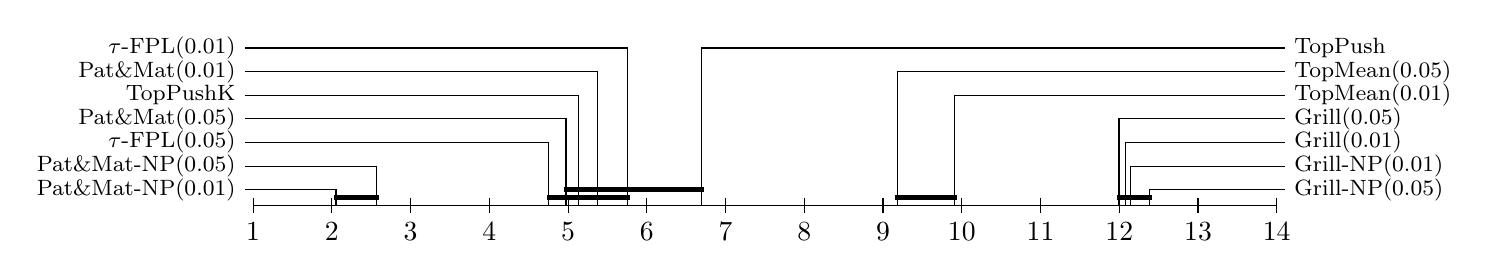
\begin{tikzpicture}[scale = 1.0]
    \draw (1.0,0) -- (14.0,0);
    \foreach \x in {1,...,14} \draw (\x,0.10) -- (\x,-0.10) node[anchor=north]{$\x$};
    \draw (2.051948051948052,0) -- (2.051948051948052,0.19999999999999998) -- (0.9, 0.19999999999999998) node[anchor=east] {\footnotesize Pat\&Mat-NP(0.01)};
    \draw (2.564935064935065,0) -- (2.564935064935065,0.5) -- (0.9, 0.5) node[anchor=east] {\footnotesize Pat\&Mat-NP(0.05)};
    \draw (4.7564935064935066,0) -- (4.7564935064935066,0.7999999999999999) -- (0.9, 0.7999999999999999) node[anchor=east] {\footnotesize $\tau$-FPL(0.05)};
    \draw (4.974025974025974,0) -- (4.974025974025974,1.0999999999999999) -- (0.9, 1.0999999999999999) node[anchor=east] {\footnotesize Pat\&Mat(0.05)};
    \draw (5.136363636363637,0) -- (5.136363636363637,1.4) -- (0.9, 1.4) node[anchor=east] {\footnotesize TopPushK};
    \draw (5.37012987012987,0) -- (5.37012987012987,1.6999999999999997) -- (0.9, 1.6999999999999997) node[anchor=east] {\footnotesize Pat\&Mat(0.01)};
    \draw (5.753246753246753,0) -- (5.753246753246753,2.0) -- (0.9, 2.0) node[anchor=east] {\footnotesize $\tau$-FPL(0.01)};
    \draw (6.694805194805195,0) -- (6.694805194805195,1.9999999999999998) -- (14.1, 1.9999999999999998) node[anchor=west] {\footnotesize TopPush};
    \draw (9.181818181818182,0) -- (9.181818181818182,1.7) -- (14.1, 1.7) node[anchor=west] {\footnotesize TopMean(0.05)};
    \draw (9.905844155844155,0) -- (9.905844155844155,1.4) -- (14.1, 1.4) node[anchor=west] {\footnotesize TopMean(0.01)};
    \draw (11.996753246753247,0) -- (11.996753246753247,1.0999999999999999) -- (14.1, 1.0999999999999999) node[anchor=west] {\footnotesize Grill(0.05)};
    \draw (12.084415584415584,0) -- (12.084415584415584,0.8) -- (14.1, 0.8) node[anchor=west] {\footnotesize Grill(0.01)};
    \draw (12.146103896103897,0) -- (12.146103896103897,0.5) -- (14.1, 0.5) node[anchor=west] {\footnotesize Grill-NP(0.01)};
    \draw (12.383116883116884,0) -- (12.383116883116884,0.2) -- (14.1, 0.2) node[anchor=west] {\footnotesize Grill-NP(0.05)};
    \draw[line width=0.06cm,color=black,draw opacity=1.0] (2.021948051948052,0.1) -- (2.594935064935065,0.1);
    \draw[line width=0.06cm,color=black,draw opacity=1.0] (4.726493506493506,0.1) -- (5.783246753246753,0.1);
    \draw[line width=0.06cm,color=black,draw opacity=1.0] (4.9440259740259735,0.2) -- (6.724805194805195,0.2);
    \draw[line width=0.06cm,color=black,draw opacity=1.0] (9.151818181818182,0.1) -- (9.935844155844155,0.1);
    \draw[line width=0.06cm,color=black,draw opacity=1.0] (11.966753246753248,0.1) -- (12.413116883116883,0.1);
  \end{tikzpicture}
}

    \vspace{-9mm}
    \caption{Critical difference (CD) diagrams (level of importance 0.05) of the Nemenyi post hoc test for the Friedman test. Each diagram shows the mean rank of each method, with rank 1 being the best. Black wide horizontal lines group together methods with the mean ranks that are not significantly different. The critical difference diagrams were computed for mean rank averages over all datasets of the tpr@fpr ($\tau=0.01$) metric.}
    \label{fig:cd1}
\end{figure}

\begin{figure}[!ht]
    \centering
    \documentclass[tikz]{standalone}
\usepackage[ddmmyyyy]{datetime}

% ------------------------------------------------------------------------------
% Packages
% ------------------------------------------------------------------------------
% Page setting
\usepackage[explicit]{titlesec}
\usepackage{sectsty}
\usepackage{fancyhdr}

% Text options
\usepackage{lmodern}
\usepackage[T1]{fontenc}
\usepackage[utf8]{inputenc}
\usepackage{xspace}

\usepackage{amsfonts}
\usepackage{dsfont}
\usepackage{pifont}

\usepackage[color=myred!50]{todonotes}

% Graphics and colors
\usepackage{graphicx}
\usepackage{import}
\usepackage{graphics}
\usepackage{xcolor}

\definecolor{myred}{RGB}{150,0,0}  
\definecolor{mygreen}{RGB}{0,150,0}
\definecolor{myblue}{RGB}{0, 101, 189}
\definecolor{myyellow}{RGB}{220, 206, 0}
\definecolor{myorange}{RGB}{255, 153, 51}
\definecolor{mycyan}{RGB}{51, 204, 204}
\definecolor{mypurple}{RGB}{204, 0, 153}

\newcommand{\doccol}{\color{myblue}}

% Hyperrefs
\usepackage{hyperref}
\hypersetup{
  pdfusetitle,
  unicode = true,
  bookmarks = true,
  bookmarksnumbered = false,
  bookmarksopen = true,
  breaklinks = false,
  pdfborderstyle = {},
  backref = false,
  colorlinks = true,
  linkcolor = myblue,
  urlcolor = myred,
  citecolor = mygreen,
}

% enumerate and itemize
\usepackage{enumitem}

% Appendix
\usepackage[title, titletoc]{appendix}

% Captions
\usepackage{caption}
\usepackage{subcaption}

\captionsetup[figure]{position = bottom}
\captionsetup[table]{position = bottom}

% Figures

% Tables
\usepackage{booktabs}
\usepackage{nicematrix}

\renewcommand{\arraystretch}{1.5}

% Algorithms
\usepackage{algorithm}
\usepackage{algorithmicx}
\usepackage{algpseudocode}

% Math
\usepackage{amsmath}
\usepackage{amsthm}
\usepackage{amssymb}
\usepackage{mathtools}
\usepackage{nicefrac}
\usepackage{bm}
\usepackage{thmtools}
\usepackage{thm-restate}
\usepackage{optidef}

% Theorems
\usepackage[framemethod=TikZ]{mdframed}
\usepackage{xifthen}

% Tikz and pfgplots
\usepackage{tikz}
\usepackage{pgfplots}
\usepackage{pgfplotstable}

\usetikzlibrary{shapes}
\usetikzlibrary{arrows}
\usetikzlibrary{automata}
\usetikzlibrary{positioning}
\usetikzlibrary{calc}
\usetikzlibrary{intersections}

\pgfplotsset{compat=newest}
\usepgfplotslibrary{groupplots}
\usepgfplotslibrary{fillbetween}

% ------------------------------------------------------------------------------
% Math declarations
% ------------------------------------------------------------------------------
\newcommand{\Brac}[2][r]{%
  \ifx r#1 \left(       #2 \right)       \else
  \ifx c#1 \left\{      #2 \right\}      \else
  \ifx s#1 \left[       #2 \right]       \else
  \ifx v#1 \left\vert   #2 \right\vert   \else
  \ifx a#1 \left\langle #2 \right\rangle \else
  \ifx t#1 \left\lceil  #2 \right\rceil  \else
  \ifx b#1 \left\lfloor #2 \right\rfloor \else
  \ifx n#1 \left\|      #2 \right\|      \else
  \mathrm{Illegal~option}%
  \fi\fi\fi\fi\fi\fi\fi\fi
}

\newcommand{\clip}[4][s]{
  \ifx s#1 \mathrm{clip}_{\Brac[s]{#2,\; #3}}\Brac{#4} \else
  \ifx u#1 \mathrm{clip}_{\left[#2,\; #3\right)}\Brac{#4} \else
  \ifx l#1 \mathrm{clip}_{\left(#2,\; #3\right]}\Brac{#4} \else
  \mathrm{Illegal~option}%
  \fi\fi\fi
}

\newcommand{\yesmark}{\textcolor{mygreen}{\ding{51}}}%
\newcommand{\nomark}{\textcolor{myred}{\ding{55}}}
\newcommand{\good}[1]{\textcolor{mygreen}{#1}}
\newcommand{\bad}[1]{\textcolor{myred}{#1}}

\newcommand{\R}{\mathbb{R}}
\newcommand{\N}{\mathbb{N}}
\newcommand{\X}{\mathbb{X}}
\newcommand{\Xc}{\mathcal{X}}
\newcommand{\D}{\mathcal{D}}

\newcommand{\I}{\mathcal{I}}
\newcommand{\Itil}{\tilde{\mathcal{I}}}
\newcommand{\Ineg}{\I_{-}}
\newcommand{\Ipos}{\I_{+}}

\newcommand{\Imb}{\I_{\text{mb}}}
\newcommand{\Imbneg}{\I_{\text{mb},-}}
\newcommand{\Imbpos}{\I_{\text{mb},+}}

\newcommand{\nall}{n}
\newcommand{\nneg}{n_{-}}
\newcommand{\npos}{n_{+}}
\newcommand{\ntil}{\tilde{n}}

\newcommand{\nmb}{n_{\text{mb}}}
\newcommand{\nmbneg}{n_{\text{mb},-}}
\newcommand{\nmbpos}{n_{\text{mb},+}}

\newcommand{\K}{\mathbb{K}}
\newcommand{\Kall}{\K^{\pm}}
\newcommand{\Kneg}{\K^{-}}

\newcommand{\updateaa}{\Delta_{\alpha,\alpha}}
\newcommand{\updateab}{\Delta_{\alpha,\beta}}
\newcommand{\updatebb}{\Delta_{\beta,\beta}}

\newcommand{\alphak}{\alpha_{\hat{k}}}
\newcommand{\alphal}{\alpha_{\hat{l}}}
\newcommand{\betak}{\beta_{\hat{k}}}
\newcommand{\betal}{\beta_{\hat{l}}}

\newcommand{\norm}[1]{\Brac[n]{#1}}
\newcommand{\abs}[1]{|#1|}
\newcommand{\inner}[2]{\Brac[a]{#1, \; #2}}
\newcommand{\dd}[1]{\mathop{}\!\mathrm{d}#1}
\newcommand{\minimize}[1]{\ifthenelse{\isempty{#1}}{\operatorname*{minimize}\quad}{\operatorname*{minimize}_{#1}\quad}}
\newcommand{\maximize}[1]{\ifthenelse{\isempty{#1}}{\operatorname*{maximize}\quad}{\operatorname*{maximize}_{#1}\quad}}
\newcommand{\st}{\operatorname{subject\ to}}
\newcommand{\argmin}{\operatorname*{argmin}}
\newcommand{\eps}{{\varepsilon}}

\newcommand{\Imin}{I_{\rm mb}}
\newcommand{\Iminh}{I_{\rm mb}^{\rm enh}}
\newcommand{\nmin}{n_{\rm mb}}
\newcommand{\II}{\mathds{1}}
\newcommand{\Iverson}[1]{\mathds{1}_{\Brac[s]{#1}}}

\newcommand{\EE}{\mathbb{E}}
\newcommand{\PP}{\mathbb{P}}
\newcommand{\bias}{\operatorname{bias}}

\newcommand{\Matrix}[1]{\begin{pmatrix} #1 \end{pmatrix}}
\newcommand{\Set}[2]{\Brac[c]{#1 \; \middle\vert \; #2}}
\newcommand{\domain}{\operatorname*{dom}}

\newcommand{\repeatloop}{\texttt{repeat}\xspace}
\newcommand{\forloop}{\texttt{for}\xspace}

\newcommand{\vecab}{\Matrix{\bm{\alpha} \\ \bm{\beta}}}

% models
\newcommand{\AccatTop}{\emph{Accuracy at the Top}\xspace}
\newcommand{\TopPush}{\emph{TopPush}\xspace}
\newcommand{\TopPushK}{\emph{TopPushK}\xspace}
\newcommand{\tauFPL}{{\emph{$\tau$-FPL}}\xspace}
\newcommand{\TopMeanK}{\emph{TopMeanK}\xspace}
\newcommand{\PatMat}{\emph{Pat}\&\emph{Mat}\xspace}
\newcommand{\PatMatNP}{{\emph{Pat}\&\emph{Mat-NP}}\xspace}
\newcommand{\Grill}{\emph{Grill}\xspace}
\newcommand{\GrillNP}{\emph{Grill-NP}\xspace}
\newcommand{\DeepTopPush}{\emph{DeepTopPush}\xspace}
\newcommand{\TFCO}{\emph{TFCO}\xspace}
\newcommand{\APPerf}{\emph{Ap-Perf}\xspace}
\newcommand{\BaseLine}{\emph{BaseLine}\xspace}

% counts and rates
\DeclareMathOperator{\tp}{tp}
\DeclareMathOperator{\tn}{tn}
\DeclareMathOperator{\fp}{fp}
\DeclareMathOperator{\fn}{fn}
\DeclareMathOperator{\tpr}{tpr}
\DeclareMathOperator{\tnr}{tnr}
\DeclareMathOperator{\fpr}{fpr}
\DeclareMathOperator{\fnr}{fnr}

\DeclareMathOperator{\tps}{\overline{tp}}
\DeclareMathOperator{\tns}{\overline{tn}}
\DeclareMathOperator{\fps}{\overline{fp}}
\DeclareMathOperator{\fns}{\overline{fn}}

\DeclareMathOperator{\accuracy}{acc}
\DeclareMathOperator{\baccuracy}{bacc}
\DeclareMathOperator{\precision}{precision}
\DeclareMathOperator{\recall}{recall}
\DeclareMathOperator{\pratrec}{Precision@Recall}
\DeclareMathOperator{\postop}{pos@top}

% ------------------------------------------------------------------------------
% Document
% ------------------------------------------------------------------------------
\begin{document}
% 
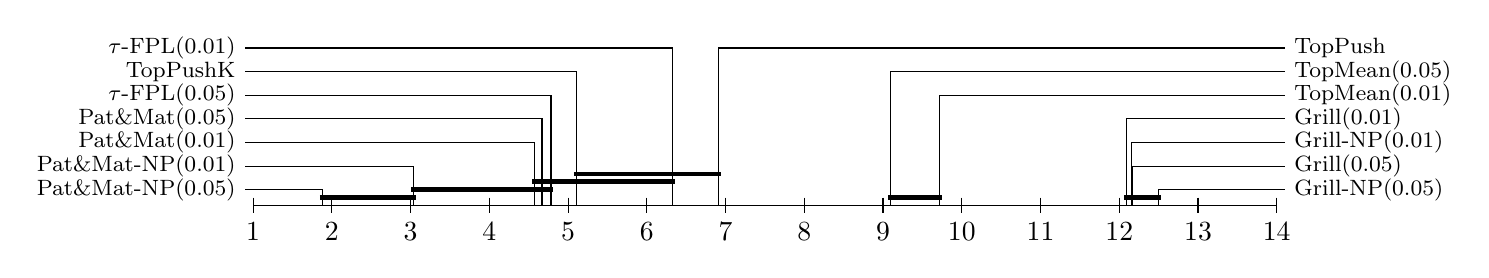
\begin{tikzpicture}
  \draw (1.0,0) -- (14.0,0);
  \foreach \x in {1,...,14} \draw (\x,0.10) -- (\x,-0.10) node[anchor=north]{$\x$};   \draw (1.8766233766233766,0) -- (1.8766233766233766,0.19999999999999998) -- (0.9, 0.19999999999999998) node[anchor=east] {\footnotesize Pat\&Mat-NP(0.05)};
  \draw (3.0357142857142856,0) -- (3.0357142857142856,0.5) -- (0.9, 0.5) node[anchor=east] {\footnotesize Pat\&Mat-NP(0.01)};
  \draw (4.577922077922078,0) -- (4.577922077922078,0.7999999999999999) -- (0.9, 0.7999999999999999) node[anchor=east] {\footnotesize Pat\&Mat(0.01)};
  \draw (4.6688311688311686,0) -- (4.6688311688311686,1.0999999999999999) -- (0.9, 1.0999999999999999) node[anchor=east] {\footnotesize Pat\&Mat(0.05)};
  \draw (4.782467532467533,0) -- (4.782467532467533,1.4) -- (0.9, 1.4) node[anchor=east] {\footnotesize $\tau$-FPL(0.05)};
  \draw (5.103896103896104,0) -- (5.103896103896104,1.6999999999999997) -- (0.9, 1.6999999999999997) node[anchor=east] {\footnotesize TopPushK};
  \draw (6.327922077922078,0) -- (6.327922077922078,2.0) -- (0.9, 2.0) node[anchor=east] {\footnotesize $\tau$-FPL(0.01)};
  \draw (6.9058441558441555,0) -- (6.9058441558441555,1.9999999999999998) -- (14.1, 1.9999999999999998) node[anchor=west] {\footnotesize TopPush};
  \draw (9.097402597402597,0) -- (9.097402597402597,1.7) -- (14.1, 1.7) node[anchor=west] {\footnotesize TopMean(0.05)};
  \draw (9.714285714285714,0) -- (9.714285714285714,1.4) -- (14.1, 1.4) node[anchor=west] {\footnotesize TopMean(0.01)};
  \draw (12.090909090909092,0) -- (12.090909090909092,1.0999999999999999) -- (14.1, 1.0999999999999999) node[anchor=west] {\footnotesize Grill(0.01)};
  \draw (12.152597402597403,0) -- (12.152597402597403,0.8) -- (14.1, 0.8) node[anchor=west] {\footnotesize Grill-NP(0.01)};
  \draw (12.162337662337663,0) -- (12.162337662337663,0.5) -- (14.1, 0.5) node[anchor=west] {\footnotesize Grill(0.05)};
  \draw (12.503246753246753,0) -- (12.503246753246753,0.2) -- (14.1, 0.2) node[anchor=west] {\footnotesize Grill-NP(0.05)};
  \draw[line width=0.06cm,color=black,draw opacity=1.0] (1.8466233766233766,0.1) -- (3.0657142857142854,0.1);
  \draw[line width=0.06cm,color=black,draw opacity=1.0] (3.005714285714286,0.2) -- (4.812467532467533,0.2);
  \draw[line width=0.06cm,color=black,draw opacity=1.0] (4.5479220779220775,0.30000000000000004) -- (6.357922077922078,0.30000000000000004);
  \draw[line width=0.06cm,color=black,draw opacity=1.0] (5.073896103896104,0.4) -- (6.935844155844156,0.4);
  \draw[line width=0.06cm,color=black,draw opacity=1.0] (9.067402597402598,0.1) -- (9.744285714285713,0.1);
  \draw[line width=0.06cm,color=black,draw opacity=1.0] (12.060909090909092,0.1) -- (12.533246753246752,0.1);
\end{tikzpicture}
% 
\end{document}
    \vspace{-9mm}
    \caption{Critical difference (CD) diagrams (level of importance 0.05) of the Nemenyi post hoc test for the Friedman test. Each diagram shows the mean rank of each method, with rank 1 being the best. Black wide horizontal lines group together methods with the mean ranks that are not significantly different. The critical difference diagrams were computed for mean rank averages over all datasets of the tpr@fpr ($\tau=0.05$) metric.}
    \label{fig:cd2}
\end{figure}






From this figure and table, we make several observations:
\begin{itemize}\itemsep 0pt
\item \NEW{\toppushk (rank 5.1) provides a slight improvement over \toppush (rank 6.7) even though this improvement is not statistically significant as both methods are connected by the black line in both Figures \ref{fig:cd1} and \ref{fig:cd2}.}
\item Neither \grill \NEW{ (ranks 12.0 and 12.1)} nor \npA \NEW{ (ranks 12.1 and 12.4)} perform well. We believe this happened due to the lack of convexity as indicated in Theorem \ref{thm:convex} and the discussion after that.
\item \topmeank \NEW{ (ranks 9.2 and 9.9)} does not perform well either. Since the thresholds $\tau$ are small, then $\bm w=0$ is the global minimum as proved in Corollary \ref{cor:topmean}.
\item \npB \NEW{ (rank 2.1 and 2.6)} seems to outperform other methods.
\item \NEW{\patmat (ranks 5.0 and 5.4), \npC (ranks 4.8 and 5.8) and \toppushk (rank 5.1) perform similarly. Since they are connected, there is no statistical difference between their behaviours.}
\item \NEW{\npB at level $0.01$ (rank 2.1) outperforms \npB at level $0.05$ (rank 2.6) for $\tau=0.01$. \npB at level $0.05$ (rank 1.9 in Figure \ref{fig:cd2}) outperforms \npB at level $0.01$ (rank 3.0 in Figure \ref{fig:cd2}) for $\tau=0.05$. This should be because these methods are optimized for the corresponding threshold. For $\npC$ we observed this behaviour for Figure \ref{fig:cd2} but not for Figure \ref{fig:cd1}.}
\end{itemize}

\NEW{Figure \ref{fig:wilcoxon} provides a similar comparison. Both axes are sorted from the best (left) to the worst (right) average ranks. The numbers in the graph show the $p$-value for the pairwise Wilcoxon signed-rank test, where the null hypothesis is that the mean tpr@fpr of both methods is the same. Even though Figure \ref{fig:cd1} employs a comparison of mean ranks and Figure \ref{fig:wilcoxon} a pairwise comparison of fpr@tpr, the results are almost similar. Methods grouped by the black line in the former figure usually show a large $p$-value in the latter figure.}

\begin{figure}[!ht]
    \centering
    \includegraphics[width = \linewidth]{figures/wilcoxon_fpr_1.pdf}
    \caption{The $p$-value for the parwise Wilcoxon signed-rank test, where the null hypothesis is that the mean tpr@fpr(0.01) of both methods is the same. The methods are sorted by mean rank (left = better).}
    \label{fig:wilcoxon}
\end{figure}

Table \ref{tab:fails} investigates the impact of $\bm w=0$ as a potential global minimum. Each method was optimized for six different values of hyperparameters. The table depicts the condition under which the final value has a lower objective than $\bm w=0$. Thus, \cmark\ means that it is always better while \xmark\ means that the algorithm made no progress from the starting point $\bm w =0$. The latter case implies that $\bm w=0$ seems to be the global minimum. We make the following observations:
\begin{itemize}\itemsep 0pt
\item \patmat and \npB are the only methods which succeeded at every dataset for some hyperparameter. Moreover, for each dataset, there was some $\beta_0$ such that these methods were successful if and only if $\beta\in(0,\beta_0)$. This is in agreement with Theorem~\ref{thm:patmat_zero}.
\item \topmeank fails everywhere which agrees with Corollary \ref{cor:topmean}.
%\item \toppush has a lower number of successes than \toppushk, which corresponds to Figure \ref{fig:thresholds} showing that the latter method has a lower threshold. This holds for \toppushk and \npC as well.
\item Figure \ref{fig:thresholds} states that the methods from Section \ref{sec:obj2} has a higher threshold than their Neyman-Pearson variants from Section \ref{sec:obj3}. This is documented in the table as the latter have a higher number of successes.
\end{itemize}

\begin{table}[!ht]
\caption{Necessary hyperparameter choice for the solution to have a better objective than zero. \cmark\ means that the solution was better than zero for all hyperparameters while \xmark\ means that it was worse for all hyperparameters.}
\label{tab:fails}
\centering
\begin{tabular}{@{}lllll@{}}
\toprule
 & Ionosphere & Hepmass & FashionMNIST & CIFAR100 \\
\midrule
\atoppush						& \cmark 	&\xmark	&\cmark	&\xmark          \\
\atoppushk 						& \cmark	&\xmark	&\cmark	&\xmark                      \\
\agrill$\tau=0.01$ 				& \xmark	&\xmark	& \xmark	&\xmark              \\
\phantom{\agrill}$\tau=0.0$     & \xmark	&\xmark	& \xmark	&\xmark              \\
\apatmat$\tau=0.01$				& \cmark	&{\color{mygreen} \boldmath$\beta\le 0.1$}	&{\color{mygreen} \boldmath$\beta\le 1$}	&{\color{mygreen} \boldmath$\beta\le 1$}  \\
\phantom{\apatmat}$\tau=0.05$ 	& \cmark	&{\color{mygreen} \boldmath$\beta\le 1$}	&\cmark	& \cmark 			\\
\atopmeank$\tau=0.01$ 			& \xmark	&\xmark	&\xmark	&\xmark                      \\
\phantom{\atopmeank}$\tau=0.05$ & \xmark	&\xmark	&\xmark	&\xmark                      \\
\anpA$\tau=0.01$				& \xmark	&\xmark	&\xmark	&\xmark              \\
\phantom{\anpA}$\tau=0.05$ 		& \xmark	&\xmark	&\xmark	&\xmark                      \\
\anpB$\tau=0.01$ 				& \cmark	&{\color{mygreen} \boldmath$\beta\le 1$}	&\cmark	&{\color{mygreen} \boldmath$\beta\le 1$}        \\
\phantom{\anpB}$\tau=0.05$		& \cmark	&\cmark	&\cmark	&{\color{mygreen} \boldmath$\beta\le 1$}              \\
\anpC$\tau=0.01$ 				& \cmark	&\xmark	&\cmark	&\xmark                      \\
\phantom{\anpC}$\tau=0.05$		& \cmark	&\cmark	&\cmark	&{\color{mygreen} \boldmath$\lambda\le 0.001$}                      \\
\bottomrule
\end{tabular}
\end{table}









\section{Conclusion}

In this paper, we achieved the following results:
\begin{itemize}\itemsep 0pt
\item We presented a unified framework for the three criteria from Section \ref{sec:framework}. \NEW{These criteria include ranking, accuracy at the top and hypothesis testing.}
\item We showed that several known methods (\toppush, \grill, \npC) fall into our framework and derived some completely new methods (\patmat, \npB).
\item We performed a theoretical analysis of the methods. We showed that known methods suffer from certain disadvantages. While \toppush and \npC are sensitive to outliers, \grill is non-convex. We proved the global convergence of the stochastic gradient descent for \patmat and \npB.
\item We performed a numerical comparison and we showed a good performance of our method \npB.
\end{itemize}
%Based on the results, we recommend using \toppushk or \npC for extremely small $\tau$. For larger $\tau$, we recommend using \patmat or \npB as they are convex and do not suffer from problems at $\bm w=0$.


\section*{Acknowledgements}


This work was supported by the Grant Agency of the Czech Republic (18-21409S) and by the OP RDE (OP VVV) funded project Research Center for Informatics, reg. No: CZ02.1.01/0.0./0.0./16\_019/0000765.


\appendix


\section{Additional results and proofs}\label{app:proofs}

Here, we provide additional results and proofs of results mentioned in the main body. For convenience, we repeat the result statements.

\subsection{Equivalence of \eqref{eq:problem_aatp_orig} and \eqref{eq:problem_aatp}}

To show this equivalence, we will start with an auxiliary lemma.

\begin{lemma}\label{lemma:fnfp_equivalence}
Denote by $t$ the exact quantile from \eqref{eq:defin_quantile}. Then for all $\mu\in[0,1]$ we have
\begin{equation}\label{eq:fnfp_equivalence}
\fp (\bm w,t) = \mu \fp(\bm w,t) + (1-\mu)\fn(\bm w,t) + (1-\mu)(n\tau - n^+) + (1-\mu)(q - 1),
\end{equation}
where $q:= \#\{\bm x\in\mathcal X|\ \bm w^\top \bm x= t\}$.
\end{lemma}
\begin{proof}
By the definition of the quantile we have
$$
\tp(\bm w,t)+\fp(\bm w,t) = n\tau + q-1.
$$
This implies
$$
\fp(\bm w,t)=n\tau +q - 1-\tp(\bm w,t) =n\tau+q-1-n^{+} +\fn(\bm w,t).
$$
From this relation we deduce
$$
\aligned
\fp(\bm w,t) &= \mu \fp(\bm w,t) + (1-\mu)\fp(\bm w,t) = \mu \fp(\bm w,t) + (1-\mu)\left(\fn(\bm w,t) + n\tau - n^+ + q - 1\right)\\
&= \mu \fp(\bm w,t) + (1-\mu)\fn(\bm w,t) + (1-\mu)\left(n\tau - n^+\right) + (1-\mu)\left(q - 1\right),
\endaligned
$$
which is precisely the lemma statement.
\end{proof}


The right-hand side of \eqref{eq:fnfp_equivalence} consists of three parts. The first one is a convex combination of false-positives and false-negatives. The second one is a constant term which has no impact on optimization. Finally, the third term $(1-\mu)\left(q - 1\right)$ equals the number of samples for which their classifier equals the quantile. However, this term is small in comparison with the true-positives and the false-negatives and can be neglected. Moreover, when the data are ``truly'' random such as when measurement errors are present, then $q=1$ and this term vanishes completely. This gives the (almost) equivalence of \eqref{eq:problem_aatp_orig} and \eqref{eq:problem_aatp}. Note that term $q$ is ignored in many papers.



\subsection{Results related to convexity}


\propositionNN{prop:convex}{Thresholds $t_2$ and $t_3$ are convex functions of the weights. The threshold function $t_1$ is non-convex.}
\begin{proof}
  It is easy to show that the quantile $t_1$ is not convex. Due to \cite{lapin.2015}, the mean of the $k$ highest values of a vector is a convex function and therefore, $t_2$ is a convex function. It remains to analyze $t_3$. It is defined via an implicit equation, where we consider for simplicity $\beta=1$,
$$
g(\bm w,t):=\frac{1}{n}\sum_{\bm x\in\mathcal{X}} l(\bm w^\top \bm x-t) - \tau = 0.
$$
Since $l$ is convex, we immediately obtain that $g$ is jointly convex in both variables.

To show the convexity, consider $\bm w$, $\hat{\bm w}$ and the corresponding $t= t_3(\bm w)$, $\hat t=t_3(\hat{\bm w})$. Note that this implies $g(\bm w,t)=g(\hat{\bm w},\hat t)=0$. Then for any $\lambda\in[0,1]$ we have 
\begin{equation}\label{eq:proof_conv1}
g(\lambda\bm w+(1-\lambda)\hat{\bm w},\;\lambda t+(1-\lambda)\hat t) \le\lambda g(\bm w,t)+(1-\lambda)g(\hat{\bm w},\hat t)=0,
\end{equation}
where the inequality follows from the convexity of $g$ and the equality from $g(\bm w,t)=g(\hat{\bm w},\hat t)=0.$
From the definition of the surrogate quantile function $t_3$ we have
\begin{equation}\label{eq:proof_conv2}
g(\lambda\bm w+(1-\lambda)\hat{\bm w},t_3(\lambda\bm w+(1-\lambda)\hat{\bm w}))=0.
\end{equation}
Since $g$ is non-increasing in the second variable, from \eqref{eq:proof_conv1} and \eqref{eq:proof_conv2} we deduce
$$
t_3(\lambda\bm w+(1-\lambda)\hat{\bm w})\le\lambda t+(1-\lambda)\hat t =\lambda t_3(\bm w)+(1-\lambda) t_3(\hat{\bm w}),
$$
which implies that function $\bm w\mapsto t_3(\bm w)$ is convex.
\end{proof}




\theoremNN{thm:convex}{If the threshold $t$ is a convex function of the weights $\bm w$, then function $f(\bm w) = \fns(\bm w, t(\bm w))$ is convex.}
\begin{proof}
Due to the definition of the surrogate counts \eqref{eq:defin_counts_surr}, the objective of \eqref{eq:problem2} equals to
$$
\frac{1}{n^+}\sum_{\bm x\in\mathcal{X}^+} l\left(t(\bm w)-\bm w^\top \bm x\right).
$$
Here we write $t(\bm w)$ to stress the dependence of $t$ on $\bm w$. Since $\bm w\mapsto t(\bm w)$ is a convex function, we also have that $\bm w\mapsto t(\bm w)-\bm w^\top \bm x$ is a convex function. From its definition, the surrogate function $l$ is convex and non-decreasing. Since a composition of a convex function with a non-decreasing convex function is a convex function, this finishes the proof.
\end{proof}



\subsection{Results related to differentiability}


\theoremNN{thm:derivative}{If the surrogate function $l$ is differentiable, then threshold $t_3$ is a differentiable function of the weights $\bm w$ and its derivative equals to
  $$
    \nabla t_3(\bm w) = \frac{\sum_{\bm x\in\Xcal}l'(\beta(\bm w^\top \bm x-t_3(\bm w)))\bm x}{\sum_{\bm x\in\Xcal}l'(\beta(\bm w^\top \bm x-t_3(\bm w)))}.
  $$
  The threshold functions $t_1$ and $t_2$ are non-differentiable.}
\begin{proof}
  The result for $t_3$ follows directly from the implicit function theorem. The non-differentiability of $t_1$ and $t_2$ happens whenever the threshold value is achieved at two different scores.
\end{proof}



\subsection{Results related to stability}


\theoremNN{thm:large_t}{
Consider any of these formulations: \toppush, \toppushk, \topmeank or \npC. Fix any $\bm w$ and denote the corresponding threshold $t(\bm w)$. If we have
\begin{equation}\label{eq:w_zero_nn}
  t(\bm w)\ge \frac{1}{n^+} \sum_{\bm x^+\in\Xcal^+} \bm w^\top \bm x^+,
\end{equation}
then $f(\bm 0)\le f(\bm w)$. Specifically, denote the scores $z^+=\bm w^\top \bm x^+$ for $\bm x^+\in\Xcal^+$ and $z^-=\bm w^\top \bm x^-$ for $\bm x^-\in\Xcal^-$ and the ordered variants with decreasing components of $\bm z^-$ by $\bm z_{[\cdot]}^-$. Then
$$
\aligned
z_{[1]}^- \ge \frac{1}{n^+}\sum_{i=1}^{n^+} z_{i}^+ &\implies f(\bm 0)\le f(\bm w)\text{ for }\toppush, \\
\frac{1}{k}\sum_{i=1}^kz_{[i]}^- \ge \frac{1}{n^+}\sum_{i=1}^{n^+} z_{i}^+ &\implies f(\bm 0)\le f(\bm w)\text{ for }\toppushk, \\
\frac{1}{n^-\tau}\sum_{i=1}^{n^-\tau}z_{[i]}^- \ge \frac{1}{n^+}\sum_{i=1}^{n^+} z_{i}^+ &\implies f(\bm 0)\le f(\bm w)\text{ for }\npC. \\
\endaligned
$$
}
\begin{proof}
Due to $l(0)=1$ and the convexity of $l$ we have $l(z)\ge 1+cz$, where $c$ equals to the derivative of $l$ at $0$. Then we have
$$
\aligned
f(\bm w) &\ge \frac{1}{n^+}\fns(\bm w, t) = \frac{1}{n^+}\sum_{\bm x\in\Xcal^+}l(t-\bm w^\top \bm x) \ge \frac{1}{n^+}\sum_{\bm x\in\Xcal^+}(1+c(t-\bm w^\top \bm x)) \\
&= 1+\frac{c}{n^+}\sum_{\bm x\in\Xcal^+}(t-\bm w^\top \bm x) = 1+ct - \frac{c}{n^+}\sum_{\bm x\in\Xcal^+}\bm w^\top \bm x \ge 1,
\endaligned
$$
where the last inequality follows from \eqref{eq:w_zero_nn}. Now we realize that for any formulation from the statement, the corresponding threshold for $\bm w=0$ equals to $t=0$, and thus $f(\bm 0)=1$. But then $f(\bm 0)\le f(\bm w)$. The second part of the result follows from the form of thresholds $t(\bm w)$.
\end{proof}



\theoremNN{thm:patmat_zero}{
Consider the \patmat or \npB formulation with the hinge surrogate and no regularization. Assume that for some $\bm w$ we have
\begin{equation}\label{eq:patmat_zero_nn}
\frac{1}{n^+}\sum_{\bm x^+\in \Xcal^+}\bm w^\top \bm x^+ > \frac{1}{n^-}\sum_{\bm x^-\in \Xcal^-}\bm w^\top \bm x^-.
\end{equation}
Then there is a scaling parameter $\beta_0$ from \eqref{eq:defin_quantile0} such that $f(\bm w)<f(\bm 0)$ for all $\beta\in(0,\beta_0)$.
}
\begin{proof}
Define first
$$
\aligned
z_{\rm min} = \min_{\bm x\in \Xcal}\bm w^\top \bm x, \quad
\bar z = \frac{1}{n}\sum_{\bm x\in \Xcal}\bm w^\top \bm x , \quad
z_{\rm max} = \max_{\bm x\in \Xcal}\bm w^\top \bm x.
\endaligned
$$
Then we have the following chain of relations
\begin{equation}\label{eq:patmat_zero_aux0}
\aligned
\bar z &= \frac{1}{n}\sum_{\bm x\in\Xcal}\bm w^\top \bm x = \frac{1}{n}\sum_{\bm x\in\Xcal^+}\bm w^\top \bm x + \frac{1}{n}\sum_{\bm x\in\Xcal^-}\bm w^\top \bm x < \frac{1}{n}\sum_{\bm x\in\Xcal^+}\bm w^\top \bm x + \frac{n^-}{nn^+}\sum_{\bm x\in\Xcal^+}\bm w^\top \bm x \\
&= \frac 1n\left(1+\frac{n^-}{n^+}\right)\sum_{\bm x\in\Xcal^+}\bm w^\top \bm x = \frac 1n\frac{n^++n^-}{n^+}\sum_{\bm x\in\Xcal^+}\bm w^\top \bm x = \frac 1{n^+}\sum_{\bm x\in\Xcal^+}\bm w^\top \bm x.
\endaligned
\end{equation}
The only inequality follows from \eqref{eq:patmat_zero_nn} and the last equality follows from $n^++n^-=n$.

Due to \eqref{eq:patmat_zero_nn} we have $z_{\rm min}<\bar z<z_{\rm max}$. Then we can define
$$
\beta_0 = \min\left\{\frac{\tau}{\bar z-z_{\rm min}}, \frac{1-\tau}{z_{\rm max}-\bar z}, \tau\right\},
$$
observe that $\beta_0>0$, fix any $\beta\in(0,\beta_0)$ and define
$$
  t = \frac{1-\tau}{\beta_0} + \bar z.
$$
Then we obtain
\begin{equation}\label{eq:patmat_zero_aux1}
1+\beta(\bm w^\top\bm x-t) \ge 1+\beta(z_{\rm min}-t) = 1+\beta z_{\rm min}-1+\tau - \beta\bar z = \beta (z_{\rm min}-\bar z)+\tau\ge 0.
\end{equation}
Here, the first equality follows from the definition of $t$ and the last inequality from the definition of $\beta_0$. Moreover, we have
$$
\aligned
\frac{1}{n}\sum_{\bm x\in\Xcal}l(\beta(\bm w^\top\bm x-t)) &= \frac{1}{n}\sum_{\bm x\in\Xcal}\max\{1+\beta(\bm w^\top\bm x-t), 0\} = \frac{1}{n}\sum_{\bm x\in\Xcal}\left(1+\beta(\bm w^\top\bm x-t)\right) \\
&= 1-\beta t + \frac{\beta}{n}\sum_{\bm x\in\Xcal}\bm w^\top\bm x = 1-\beta t + \beta\bar z = \tau,
\endaligned
$$
where the second equality employs \eqref{eq:patmat_zero_aux1}, the third one the definition of $\bar z$ and the last one the definition of $t$. But this means that $t$ is the threshold corresponding to $\bm w$.

Similarly to \eqref{eq:patmat_zero_aux1} we get
\begin{equation}\label{eq:patmat_zero_aux2}
1+t-\bm w^\top \bm x \ge 1+t-z_{\rm max} = 1+\frac{1-\tau}{\beta} + \bar z - z_{\rm max} \ge \frac{1-\tau}{\beta} + \bar z - z_{\rm max} \ge0,
\end{equation}
where the last inequality follows from the definition of $\beta_0$. Then for the objective we have
$$
\aligned
f(\bm w) &= \frac{1}{n^+}\sum_{\bm x\in\Xcal^+}l(t-\bm w^\top \bm x) = \frac{1}{n^+}\sum_{\bm x\in\Xcal^+}\max\{1+t-\bm w^\top \bm x,0\} = \\
&= \frac{1}{n^+}\sum_{\bm x\in\Xcal^+}\left(1+t-\bm w^\top \bm x\right) =1+t-\frac{1}{n^+}\sum_{\bm x\in\Xcal^+}\bm w^\top \bm x < 1+t-\bar z \\
& = 1+\frac{1-\tau}{\beta} + \bar z -\bar z = 1+\frac{1-\tau}{\beta} = f(\bm 0),\\
\endaligned
$$
where we the third equality follows from \eqref{eq:patmat_zero_aux2}, the only inequality from \eqref{eq:patmat_zero_aux0} and the last equality from Appendix \ref{app:example}. Thus, we finished the proof for \patmat. The proof for \npB can be performed in an identical way by replacing in the definition of $\bar z$ the mean with respect to all samples by the mean with respect to all negative samples.
\end{proof}



\subsection{Results related to threshold comparison}\label{app:relations}


\begin{lemma}\label{lemma:thresholds2}
Define vector $\bm z^+$ with components $z^+=\bm w^\top \bm x^+$ for $\bm x^+\in\Xcal^+$ and similarly define vector $\bm z^-$ with components $z^-=\bm w^\top \bm x^-$ for $\bm x^-\in\Xcal^-$. Denote by $\bm z_{[\cdot]}^+$ and $\bm z_{[\cdot]}^-$ the sorted versions of $\bm z^+$ and $\bm z^-$, respectively. Then we have the following statements:
$$
\aligned
z_{[n^+\tau]}^+ > z_{[n^-\tau]}^- &\implies \grill\text{ has larger threshold than }\npA, \\
\frac{1}{n^+\tau}\sum_{i=1}^{n^+\tau} z_{[i]}^+ > \frac{1}{n^-\tau}\sum_{i=1}^{n^-\tau} z_{[i]}^-  &\implies \topmeank\text{ has larger threshold than }\npC. \\
\endaligned
$$
\end{lemma}
\begin{proof}
Since $\bm z^+$ and $\bm z^-$ are computed on disjunctive indices, we have
$$
z_{[n\tau]} \ge \min\{z_{[n^+\tau]}^+, z_{[n^-\tau]}^-\}.
$$
Since $z_{[n\tau]}$ is the threshold for \grill and $z_{[n^-\tau]}^-$ is the threshold for \npA, the first statement follows. The second part can be shown in a similar way.
\end{proof}

\noindent Since the goal of the presented formulations is to push $z^+$ above $z^-$, we may expect that the conditions in Lemma \ref{lemma:thresholds2} hold true. 



\section{Computation for Section \ref{sec:example}}\label{app:example}




\begin{comment}
Consider first solution $\bm w_1=(0,0)$. It is obvious that $\bm w_1^\top \bm x=0$ for all $\bm x$ and thus for the threshold we have $t=0$ for all formulations with the exception of \patmat where $t=\frac{1}{\beta}(1-\tau)$. The objective then equals to $f(\bm w_1)=1+t$ for all formulation with the exception of \grill where we need to add the false-positives to obtain $f(\bm w_1)=2$.

Consider now solution $\bm w_2=(1,0)$. Since the \toppush formulation chooses the largest negative, it sets $t=2$. \toppushk chooses the $k^{\rm th}$ largest negative and sets $t=\frac2k$. \grill selects the $\tau$-top quantile, which for the uniform distribution on the interval $[-1,1]$ equals to $t=1-2\tau$. For the \patmat formulation, it can be computed that for $\beta\le\tau$ we have $t=\frac{1}{\beta}(1-\tau)$ and finally \topmeank computes the average between the true quantile $1-2\tau$ and the upper bound $1$ and thus $t=1-\tau$. The objective then equals to $f(\bm w_2)=0.5+t$ for all formulation with the exception of \grill where we have to add the false-positives to get $f(\bm w_2)=0.5+t+0.5(1-t)^2$.
\end{comment}



We derive the results presented in Section \ref{sec:example} more properly. We recall that we have $n$ negative samples randomly distributed in $[-1,0]\times[-1,1]$, $n$ positive samples randomly distributed in $[0,1]\times[-1,1]$ and one negative sample at $(2,0)$. We assume that $n$ is large and the outlier may be ignored for the computation of thresholds which require a large number of points. Since the computation is simple for other formulations, we show it only for \patmat.

For $\bm w_0=(0,0)$, we get
$$
\tau = \frac{1}{n}\sum_{\bm x\in\Xcal}l(\beta(\bm w_0^\top \bm x-t)) = l(0-\beta t) = 1-\beta t,
$$
which implies $t=\frac{1}{\beta}(1-\tau)$ and consequently
$$
\frac{1}{n^+}\fns(\bm w_0,t) = \frac{1}{n^+}\sum_{\bm x\in \Xcal^+} l(t-0) = l(t) = 1+t.
$$
This finishes the computation for $\bm w_0$.

For $\bm w_1=(1,0)$ the computation goes similar. Then $\bm w_1^\top \bm x^+$ has the uniform distribution on $[0,1]$ while $\bm w_1^\top \bm x$ has the uniform distribution on $[-1,1]$. If $\beta\le\tau$, then
\begin{equation}\label{eq:example1}
\aligned
\tau &= \frac{1}{n}\sum_{\bm x\in\Xcal}l(\bm w_1^\top \bm x-t) \approx \frac12\int_{-1}^1 l(z-t)dz = \frac12\int_{-1}^1 \max\{0,1+\beta(z-t)\}dz \\
&=\frac12\int_{-1}^1 \left(1+\beta(z-t)\right)dz = 1-\beta t + \frac{\beta}{2}\int_{-1}^1zdz = 1-\beta t,
\endaligned
\end{equation}
and thus again $t=\frac{1}{\beta}(1-\tau)$. Note that
$$
1+\beta(z-t) \ge 1+\beta(-1-t) = 1-\beta - 1+\tau = -\beta+\tau \ge0
$$
and we could have ignored the $\max$ operator in \eqref{eq:example1}. Finally, we have
$$
\frac{1}{n^+}\fns(\bm w_1,t) \approx \int_0^1 l(t-z)dz = \int_0^1 \left(1+t-z\right)dz = 0.5+t.
$$


\section{Computing the threshold for \apatmat}\label{app:threshold}


We show how to efficiently compute the threshold \eqref{eq:defin_quantile0} for \patmat and the hinge surrogate~\eqref{eq:defin_surrogate}. As always define the scores $z_i=\bm w^\top \bm x_i$ and consider function
\begin{equation}\label{eq:defin_h}
h(t) = \sum_{i=1}^nl(\beta(z_i-t)) - n\tau.
\end{equation}
Then solving \eqref{eq:update_t} is equivalent to looking for $\hat t$ such that $h(\hat t)=0$. We have the following properties of $h$.

\begin{lemma}
Function $h$ is continuous and strictly decreasing (until it hits the global minimum) with $h(t)\to \infty$ as $t\to-\infty$ and $h(t)\to -n\tau$ as $t\to\infty$. Thus, there is a unique solution to the equation $h(t)=0$.
\end{lemma}

For sorted data, the following lemma gives advice on how to solve equation $h(t)=0$. 


\begin{lemma}
Let $z_1\le z_2\le\dots\le z_n$ be sorted. Define $\gamma=\frac1\beta$. Then 
\begin{equation}\label{eq:update_h}
h(z_i+\gamma) = h(z_{i+1}+\gamma) + (n-i)\beta(z_{i+1}-z_i)
\end{equation}
for all $i=n-1,\dots,1$ with the initial condition $h(z_n+\gamma)=-n\tau$.
\end{lemma}
\begin{proof}
Observe first that
$$
h(z_j+\gamma) = \sum_{i=1}^n l(\beta(z_i-z_j-\gamma)) - n\tau = \sum_{i=1}^n\max(0,\beta(z_i-z_j)) - n\tau = \sum_{i=j+1}^n \beta(z_i-z_j) - n\tau.
$$
From here, we obtain $h(z_n+\gamma)=-n\tau$. Moreover, we have
$$
\aligned
h(z_j+\gamma) &= \sum_{i=j+1}^n \beta(z_i-z_j) - n\tau = \sum_{i=j+2}^n \beta(z_i-z_{j}) + \beta(z_{j+1}-z_{j})- n\tau\\
&= \sum_{i=j+2}^n \beta(z_i-z_{j+1}) + \sum_{i=j+2}^n\beta(z_{j+1}-z_j) + \beta(z_{j+1}-z_{j})- n\tau \\
&= \sum_{i=j+2}^n \beta(z_i-z_{j+1}) + (n-j)\beta(z_{j+1}-z_j)- n\tau \\
&= h(z_{j+1}+\gamma) + (n-j)\beta(z_{j+1}-z_j),
\endaligned
$$
which finishes the proof.
\end{proof}

Thus, to solve $h(t)=0$ with the hinge surrogate, we start with $t_n=z_n+\gamma$ and $h(t_n)=-n\tau$. Then we start decreasing $t$ according to \eqref{eq:update_h} until we find some $t_i=z_i+\gamma$ such that $h(t_i)>0$. The desired $t$ then lies between $t_i$ and $t_{i+1}$. Since $h$ is a piecewise linear function with
$$
h(t) = h(t_i) + \frac{t-t_i}{t_{i+1}-t_i}\big(h(t_{i+1})-h(t_i)\big)
$$
for $t\in [t_i,t_{i+1}]$, the precise value of $\hat t$ can be computed by a simple interpolation
$$
\hat t = t_i - h(t_i)\frac{t_{i+1}-t_i}{h(t_{i+1})-h(t_i)} = t_i - h(t_i)\frac{t_{i+1}-t_i}{-(n-i)\beta(t_{i+1}-t_{i})} = t_i + \frac{h(t_i)}{\beta(n-i)}.
$$



\section{Proof of Theorem \ref{thm:sgd}}

The proof is divided into three parts. In Section \ref{app:sgd1}, we prove a general statement for convergence of stochastic gradient descent with a convex objective. In Section \ref{app:sgd2} we apply it to Theorem \ref{thm:sgd}. The proof is based on auxiliary results from Section \ref{app:sgd3}.

\subsection{General result}\label{app:sgd1}

Consider a differentiable objective function $f$ and the optimization method
\begin{equation}\label{eq:update}
w^{k+1}=w^k-\alpha^kg(w^k),
\end{equation}
where $\alpha^k>0$ is a stepsize and $g(w^k)$ is an approximation of the gradient $\nabla f(w^k)$. Assume the following:
\begin{enumerate}[label=(A\arabic*)]\itemsep 0pt
\item \label{ass_convex} $f$ is differentiable, convex and attains a global minimum;
\item \label{ass_gbound} $\norm{g(w^k)}\le B$ for all $k$;
\item \label{ass_alpha1} the stepsize is non-increasing and satisfies $\sum_{k=0}^\infty \alpha^k=\infty$;
\item \label{ass_alpha2} the stepsize satisfies $\sum_{k=0}^\infty (\alpha^k)^2<\infty$;
\item \label{ass_alpha3} the stepsize satisfies $\sum_{k=0}^\infty \nrm{\alpha^{k+1}-\alpha^k}<\infty$.
\end{enumerate}
Assumptions \ref{ass_alpha1}-\ref{ass_alpha3} are satisfied for example for $\alpha^k=\alpha^0\frac{1}{k+1}$. We start with the general result.

\begin{theorem}\label{thm:convergence}
Assume that \ref{ass_convex}-\ref{ass_alpha2} is satisfied. If there exists some $C$ such that for some global minimum of $w^*$ of $f$ we have
\begin{equation}\label{eq:nec_cond}
\sum_{k=0}^\infty\alpha^k\langle g(w^k)-\nabla f(w^k),w^*-w^k\rangle\le C,
\end{equation}
then the sequence $\{w^k\}$ generated by \eqref{eq:update} is bounded and $f(w^k)\to f(w^*)$. Thus, all its convergent subsequences converge to some global minimum of $f$.
\end{theorem}
\begin{proof}
Note first that the convexity from \ref{ass_convex} implies
\begin{equation}\label{eq:convex_estimate}
\langle \nabla f(w^k),w^*-w^k\rangle\le f(w^*)-f(w^k).
\end{equation}
Then we have
$$
\aligned
\norm{w^{k+1}-w^*}^2 &= \norm{w^k-\alpha^kg(w^k)-w^*}^2 \\
&=\norm{w^k-w^*}^2 + 2\alpha^k\langle g(w^k),w^*-w^k\rangle + (\alpha^k)^2\norm{g(w^k)}^2 \\
&\le \norm{w^k-w^*}^2 + 2\alpha^k\langle g(w^k)-\nabla f(w^k),w^*-w^k\rangle + 2\alpha^k(f(w^*)-f(w^k)) + (\alpha^k)^2B^2,
\endaligned
$$
where the inequality follows from \eqref{eq:convex_estimate} and assumption \ref{ass_gbound}. Summing this expression for all $k$ and using \eqref{eq:nec_cond} leads to
$$
\aligned
\limsup_k\norm{w^k-w^*}^2 &\le \norm{w^0-w^*}^2 +2C + 2\sum_{k=0}^\infty\alpha^k(f(w^*)-f(w^k)) + \sum_{k=0}^\infty(\alpha^k)^2B^2.
\endaligned
$$
Using assumption \ref{ass_alpha2} results in the existence of some $\hat C$ such that
\begin{equation}\label{eq:general_bound}
\limsup_k\norm{w^k-w^*}^2 + 2\sum_{k=0}^\infty\alpha^k(f(w^k) - f(w^*)) \le 2\hat C.
\end{equation}
Since $\alpha^k>0$ and $f(w^k)\ge f(w^*)$ as $w^*$ is a global minimum of $f$, we infer that sequence $\{w^k\}$ is bounded and \eqref{eq:general_bound} implies
$$
\sum_{k=0}^\infty\alpha^k(f(w^k) - f(w^*)) \le \hat C.
$$
Since $f(w^k)-f(w^*)\ge 0$, due to assumption \ref{ass_alpha1} we obtain $\lim f(w^k)\to f(w^*)$, which implies the theorem statement.
\end{proof}

\begin{comment}
Note that \eqref{eq:nec_cond} is satisfied if $\{w^k\}$ is bounded and if
\begin{equation}\label{eq:nec_cond2}
\norm{g(w^k)-\nabla f(w^k)}\le \hat C\alpha^k
\end{equation}
for some constant $\hat C$. Indeed, we have
$$
\sum_{k=0}^\infty\alpha^k\langle g(w^k)-\nabla f(w^k),w^*-w^k\rangle\le \sum_{k=0}^\infty\alpha^k \norm{g(w^k)-\nabla f(w^k)}\norm{w^*-w^k} \le 
\sum_{k=0}^\infty\alpha^k \hat C\alpha^k \norm{w^*-w^k}, 
$$
which is bounded due to \ref{ass_alpha2} and the assumed boundedness of $\{w^k\}$. Thus, condition \eqref{eq:nec_cond} states that update \eqref{eq:update} will converge whenever $g(w^k)$ lies close to the true gradient $\nabla f(w^k)$.
\end{comment}






\subsection{Proof of Theorem \ref{thm:sgd}}\label{app:sgd2}


For the proof, we will consider a general surrogate which satisfies:
\begin{enumerate}[label=(S\arabic*)]\itemsep 0pt
\item \label{surr_basic1} $l(z)\ge 0$ for all $z\in\R$,\ $l(0)=1$ and $l(z)\to 0$ as $z\to-\infty$;
\item \label{surr_basic2} $l$ is convex and strictly increasing function on $(z_0,\infty)$, where $z_0:=\sup\{z\mid l(z)=0\}$;
\item \label{surr_ratio} $\frac{l'}{l}$ is a decreasing function on $(z_0,\infty)$;
\item \label{surr_der1} $l'$ is a bounded function;
\item \label{surr_der2} $l'$ is a Lipschitz continuous function with modulus $L$.
\end{enumerate}
All these reguirements are satisfied for the surrogate logistic or by the Huber loss, which is the hinge surrogate which is smoothened on an $\eps$-neighborhood of zero.

\vspace{2mm}

\theoremNN{thm:sgd}{
  Consider the \apatmat or \anpB formulation, stepsizes $\alpha^k=\frac{\alpha^0}{k+1}$ and piecewise disjoint minibatches $I^1,\dots,I^s$ which cycle periodically $I^{k+s}=I^k$. If $l$ is the smoothened (Huberized) hinge function, then Algorithm \ref{alg:sgd} converges to the global minimum of \eqref{eq:problem_patmat}.  
}
\begin{proof}
We intend to apply Theorem \ref{thm:convergence} and thus, we need to verify its assumptions. Assumption \ref{ass_convex} is satisfied as $f$ is convex due to Theorem \ref{thm:convex}. Assumption \ref{ass_gbound} follows directly from Lemma \ref{lemma:bound_g}. Assumptions \ref{ass_alpha1},\ref{ass_alpha2} and \ref{ass_alpha3} are imposed directly in the statement of this theorem. It remains to verify \eqref{eq:nec_cond}.

For simplicity, we will do so only for $\beta=1$ and for $s=2$ minibatches of the same size. However, the proof would be identical for other values. This implies that there are some $I^k$ and $I^{k+1}$ which are pairwise disjoint, they cover all samples and that $I^k=I^{k+2}$ for all $k$. The assumptions imply that the number of positive samples in each minibatch equal to $n_+^k=\frac{1}{2}n_+$, where $n_+$ is the total number of positive samples.

First we estimate the difference between $z_i^k$ defined in \eqref{eq:defin_z} and $x_i^\top w^k$. For any $i\in I^k$ due to the construction \eqref{eq:defin_z} we have
\begin{equation}\label{eq:sgd_estimate_z1}
\aligned
z_i^k &= x_i^\top w^k, \\
z_i^{k-1} &= z_i^{k-2} = x_i^\top w^{k-2} = x_i^\top \big(w^k + \alpha^{k-2}g(w^{k-2}) + \alpha^{k-1}g(w^{k-1})\big) \\
&= x_i^\top w^k + \alpha^{k-2}x_i^\top g(w^{k-2}) + \alpha^{k-1}x_i^\top g(w^{k-1}).
\endaligned
\end{equation}
Similarly, for $i\notin I^k$ we have
\begin{equation}\label{eq:sgd_estimate_z2}
z_i^k=z_i^{k-1}=x_i^\top w^{k-1} = x_i^\top (w^k+\alpha^{k-1}g(w^{k-1})) = x_i^\top w^k + \alpha^{k-1}x_i^\top g(w^{k-1}).
\end{equation}
Recall that we already verified \ref{ass_convex}-\ref{ass_alpha3}. Combining \ref{ass_gbound} with \eqref{eq:sgd_estimate_z1} and \eqref{eq:sgd_estimate_z2} yields the existence of some $C_2$ such that for all $i\in X$ we have
\begin{equation}\label{eq:estimate_diff_z}
\aligned
\nrm{z_i^k - x_i^\top w^k} &\le C_2\alpha^{k-1}, \\
\nrm{z_i^{k-1} - x_i^\top w^k} &\le C_2\big(\alpha^{k-1}+\alpha^{k-2}\big). \\
\endaligned
\end{equation}
This also immediately implies
\begin{equation}\label{eq:estimate_diff_t}
\aligned
\nrm{t^k - t(w^k)} &\le C_2\alpha^{k-1}, \\
\nrm{t^{k-1} - t(w^k)} &\le C_2\big(\alpha^{k-1}+\alpha^{k-2}\big). \\
\endaligned
\end{equation}

Since $l'$ is Lipschitz continuous with modulus $L$ according to \ref{surr_der2}, due to \eqref{eq:estimate_diff_z} and \eqref{eq:estimate_diff_t} we get
\begin{equation}\label{eq:sgd_lipschitz1}
\aligned
\nrm{l'(t^k-z_i^k) - l'(t(w^k)-x_i^\top w^k)}&\le L \nrm{t^k-z_i^k - t(w^k)+ x_i^\top w^k} \le  2C_2L\alpha^{k-1}.
\endaligned
\end{equation}
In an identical way we can show
\begin{equation}\label{eq:sgd_lipschitz2}
\aligned
\nrm{l'(t^{k-1}-z_i^{k-1}) - l'(t(w^k)-x_i^\top w^k)}& \le 2C_2L\big(\alpha^{k-1}+\alpha^{k-2}\big), \\
\nrm{l'(z_i^k-t^k) - l'(x_i^\top w^k-t(w^k))}&\le 2C_2L\alpha^{k-1}, \\
\nrm{l'(z_i^{k-1}-t^{k-1}) - l'(x_i^\top w^k-t(w^k))}& \le 2C_2L\big(\alpha^{k-1}+\alpha^{k-2}\big).
\endaligned
\end{equation}
Now we need to estimate the distance between $\nabla t(w^k)$ and $\nabla t^k$. We have
\begin{equation}\label{eq:sgd_nablat}
\aligned
\nabla t^k &= \frac{\sum_{i\in I^k}l'(z_i^k-t^k)x_i + \sum_{i\in I^{k-1}}l'(z_i^{k-1}-t^{k-1})x_i}{\sum_{i\in X}l'(z_i^k-t^k)}, \\
\nabla t(w^k) &= \frac{\sum_{i\in I^k}l'(x_i^\top w^k-t(w^k))x_i + \sum_{i\in I^{k-1}}l'(x_i^\top w^k-t(w^k))x_i
}{\sum_{i\in X}l'(x_i^\top w^k-t(w^k))}.
\endaligned
\end{equation}
The first equality in \eqref{eq:sgd_nablat} follows from \eqref{eq:update_nablat} and \eqref{eq:update_a} while the second equality in \eqref{eq:sgd_nablat} follows from Theorem \ref{thm:derivative} and $X=I^k\cup I^{k-1}$. From Lemma \ref{lemma:bound_zero} we deduce that the denominators in \eqref{eq:sgd_nablat} are bounded away from zero uniformly in $k$. Assumption \ref{ass_alpha2} implies  $\alpha^k\to 0$. This allows us to use Lemma \ref{lemma:ratio} which together with \eqref{eq:sgd_lipschitz2} implies that there is some $C_3$ such that for all sufficiently large $k$ we have
\begin{equation}\label{eq:sgd_nablat_diff}
\norm{\nabla t^k - \nabla t(w^k)}\le C_3\big(\alpha^{k-1} + \alpha^{k-2}\big).
\end{equation}

Using the assumptions above, we can simplify the terms for $g(w^k)$ and $\nabla f(w^k)$ to
$$
\aligned
g(w^k) &= \frac{2}{n_+}\sum_{i\in I_+^k}l'(t^k-z_i^k)(\nabla t^k - x_i), \\
g(w^{k+1}) &= \frac{2}{n_+}\sum_{i\in I_+^{k+1}}l'(t^{k+1}-z_i^{k+1})(\nabla t^{k+1} - x_i), \\
\nabla f(w^k) &= \frac1{n_+}\sum_{i\in X_+}l'(t(w^k)-x_i^\top w^k)(\nabla t(w^k) - x_i), \\
\nabla f(w^{k+1}) &= \frac1{n_+}\sum_{i\in X_+}l'(t(w^{k+1})-x_i^\top w^{k+1})(\nabla t(w^{k+1}) - x_i).
\endaligned
$$
Due to the assumptions, we have $X_+=I_+^k\cup I_+^{k+1}$ and $\emptyset=I_+^k\cap I_+^{k+1}$, which allows us to write
\begin{subequations}\label{eq:sgd_sum}
\begin{align}
\label{eq:sgd_sum1} &\qquad\qquad n^+\Big(g(w^k)+g(w^{k+1})-\nabla f(w^k)-\nabla f(w^{k+1})\Big)\\
\label{eq:sgd_sum2} =&\sum_{i\in I_+^k}l'(t^k-z_i^k)(\nabla t^k - x_i) - \sum_{i\in I_+^k}l'(t(w^k)-x_i^\top w^k)(\nabla t(w^k) - x_i) \\
\label{eq:sgd_sum3} +&\sum_{i\in I_+^k}l'(t^k-z_i^k)(\nabla t^k - x_i) - \sum_{i\in I_+^k}l'(t(w^{k+1})-x_i^\top w^{k+1})(\nabla t(w^{k+1}) - x_i)\\
\label{eq:sgd_sum4} +&\sum_{i\in I_+^{k+1}}l'(t^{k+1}-z_i^{k+1})(\nabla t^{k+1} - x_i) - \sum_{i\in I^{k+1}_+}l'(t(w^k)-x_i^\top w^k)(\nabla t(w^k) - x_i) \\
\label{eq:sgd_sum5} +&\sum_{i\in I_+^{k+1}}l'(t^{k+1}-z_i^{k+1})(\nabla t^{k+1} - x_i)  - \sum_{i\in I_+^{k+1}}l'(t(w^{k+1})-x_i^\top w^{k+1})(\nabla t(w^{k+1}) - x_i).
\end{align}
\end{subequations}
Then relations \eqref{eq:sgd_nablat_diff} and \eqref{eq:sgd_lipschitz1} applied to Lemma \ref{lemma:product} imply
$$
\Big\| \sum_{i\in I_+^k}l'(t^k-z_i^k)(\nabla t^k - x_i) - \sum_{i\in I_+^k}l'(t(w^k)-x_i^\top w^k)(\nabla t(w^k) - x_i)\Big\| \le C_4\big(\alpha^{k-1} + \alpha^{k-2})
$$
for some $C_4$, which gives a bound for \eqref{eq:sgd_sum2}. Bound for \eqref{eq:sgd_sum5} is obtained by increasing $k$ by one. Bounds for \eqref{eq:sgd_sum3} and \eqref{eq:sgd_sum4} can be find similarly using \eqref{eq:sgd_lipschitz2}. Altogether, we showed
\begin{equation}\label{eq:nec_cond3}
\norm{g(w^k)+g(w^{k+1})-\nabla f(w^k)-\nabla f(w^{k+1})} \le C_1(\alpha^{k-2} + \alpha^{k-1} + \alpha^{k} + \alpha^{k+1})
\end{equation}
for some $C_1$.

We now estimate
\begin{subequations}\label{eq:proof_est1}
\begin{align}
\label{eq:proof_est11} \alpha^k&\langle g(w^{k})-\nabla f(w^{k}),w^*-w^{k}\rangle + \alpha^{k+1}\langle g(w^{k+1})-\nabla f(w^{k+1}),w^*-w^{k+1}\rangle \\
\label{eq:proof_est12} &= \langle g(w^{k})-\nabla f(w^{k}),\alpha^k(w^*-w^{k})\rangle + \langle g(w^{k+1})-\nabla f(w^{k+1}),\alpha^{k+1}(w^*-w^{k+1})\rangle \\
\label{eq:proof_est13} &= \langle g(w^{k})-\nabla f(w^{k}) + g(w^{k+1})-\nabla f(w^{k+1}),\alpha^k(w^*-w^{k})\rangle \\
\label{eq:proof_est14} &\qquad\qquad + \langle g(w^{k+1})-\nabla f(w^{k+1}),\alpha^{k+1}(w^*-w^{k+1})-\alpha^k(w^*-w^{k})\rangle.
\end{align}
\end{subequations}
To estimate \eqref{eq:proof_est14}, we make use of Lemma \ref{lemma:bound_g} to obtain the existence of some $C_5$ such that
\begin{equation}\label{eq:proof_est2}
\aligned
\langle g(w^{k+1})&-\nabla f(w^{k+1}),\alpha^{k+1}(w^*-w^{k+1})-\alpha^k(w^*-w^{k})\rangle \\
&\le 2B\norm{\alpha^{k+1}(w^*-w^{k+1})-\alpha^k(w^*-w^{k})} \\
&= 2B\norm{\alpha^{k+1}(w^*-w^k+\alpha^kg(w^k))-\alpha^k(w^*-w^{k})} \\
&= 2B\norm{(\alpha^{k+1}-\alpha^k)w^* + (\alpha^k-\alpha^{k+1})w^k +\alpha^k\alpha^{k+1} g(w^k)} \\
&\le C_5 \nrm{\alpha^{k+1}-\alpha^k} + C_5(\alpha^k)^2 + C_5(\alpha^{k+1})^2.
\endaligned
\end{equation}
In the last inequality we used the equality $2ab\le a^2+b^2$. To estimate \eqref{eq:proof_est13}, we can apply \eqref{eq:nec_cond3} together with the boundedness of $\{w^k\}$ to obtain the existence of some $C_6$ such that
\begin{equation}\label{eq:proof_est3}
\aligned
\langle g(w^{k})&-\nabla f(w^{k}) + g(w^{k+1})-\nabla f(w^{k+1}),\alpha^k(w^*-w^{k})\rangle \\
&\le C_6(\alpha^{k-2})^2 + C_6(\alpha^{k-1})^2 + C_6(\alpha^{k})^2 + C_6(\alpha^{k+1})^2.
\endaligned
\end{equation}
Plugging \eqref{eq:proof_est2} and \eqref{eq:proof_est3} into \eqref{eq:proof_est1} and summing the terms yields \eqref{eq:nec_cond}. Then the assumptions of Theorem \ref{thm:convergence} are verified and the theorem statement follows.
\end{proof}




\subsection{Auxiliary results}\label{app:sgd3}

\begin{lemma}\label{lemma:bound_zero}
Let $l$ satisfy \ref{surr_basic1}-\ref{surr_ratio}. Then there exists some $\hat C$ such that for all $k$ we have
$$
\aligned
\sum_{i\in X}l'(z_i^k-t^k) &\ge \hat C > 0, \\
\sum_{i\in X}l'(x_i^\top w^k-t(w^k)) &\ge \hat C > 0.
\endaligned
$$
\end{lemma}
\begin{proof}
First, we will find an upper bound of $z_i^k-t^k$. Fix any index $i_0$. Since $l$ is nonnegative due to \ref{surr_basic1}, equation \eqref{eq:update_t} implies
$$
n\tau=\sum_{i\in X}l(z_i^k-t^k) \ge l(z_{i_0}^k-t^k).
$$
Moreover, as $l$ is a strictly increasing function due to \ref{surr_basic2} and $n\tau>0$, this means 
\begin{equation}\label{eq:sigma_bound}
l^{-1}(n\tau) \ge z_{i_0}^k-t^k.
\end{equation}
Since $i_0$ was an arbitrary index, it holds true for all indices. Then \ref{surr_ratio} which leads to a further estimate
$$
\aligned
\sum_{i\in X}l'(z_i^k-t^k) &= \sum_{i\in X} l(z_i^k-t^k)\frac{l'(z_i^k-t^k)}{l(z_i^k-t^k)} \ge \sum_{i\in X} l(z_i^k-t^k)\frac{l'(l^{-1}(n\tau))}{l(l^{-1}(n\tau))} \\
&= n\tau\frac{l'(l^{-1}(n\tau))}{l(l^{-1}(n\tau))} = l'(l^{-1}(n\tau)),
\endaligned
$$
where the inequality follows from \eqref{eq:sigma_bound} and the following equality from \eqref{eq:update_t}. Due to \ref{surr_basic2} we obtain that $l'(l^{-1}(n\tau))$ is a positive number, which finishes the proof of the first part. The second part can be obtained in an identical way.
\end{proof}


\begin{lemma}\label{lemma:bound_g}
Let $l$ satisfy \ref{surr_basic1}-\ref{surr_der1}. Then there exists some $B$ such that for all $k$ we have $\norm{\nabla f(w^k)}\le B$ and $\norm{g(w^k)}\le B$.
\end{lemma}
\begin{proof}
Due to \ref{surr_der1} the derivative $l'$ is bounded by some $\hat B$. Then Theorem \ref{thm:derivative} and Lemma \ref{lemma:bound_zero} imply
$$
\norm{\nabla t(w^k)} \le \frac{\hat B\sum_{i\in X}\norm{x_i}
}{\sum_{i\in X}l'(x_i^\top w-t(w))} \le \frac{\hat B}{\hat C}\sum_{i\in X}\norm{x_i},
$$
which is independent of $k$. Then \eqref{eq:derivatives} and again the boundedness of $l'$ imply the existence of some $B$ such that $\norm{\nabla f(w^k)}\le B$ for all $k$. The proof for $g(w^k)$ can be performed identically.
\end{proof}

\begin{comment}
\begin{lemma}\label{lemma:bound_diff}
In the setting of Theorem \ref{thm:convergence2}, there is some $\hat C$ such that
$$
\aligned
\sum_{i\in I_+^k}l'(t^k-z_i^k)(\nabla t^k - x_i) - \sum_{i\in I_+^k}l'(t(w^{k+1})-x_i^\top w^{k+1})(\nabla t(w^{k+1}) - x_i) &\le \hat C\big( \alpha^{k+1}+\alpha^{k}+\alpha^{k-1}+\alpha^{k-2}\big), \\
\sum_{i\in I_+^{k+1}}l'(t^{k+1}-z_i^{k+1})(\nabla t^{k+1} - x_i) - \sum_{i\in I^{k+1}_+}l'(t(w^k)-x_i^\top w^k)(\nabla t(w^k) - x_i) &\le \hat C \big( \alpha^{k+1}+\alpha^{k}+\alpha^{k-1}+\alpha^{k-2}\big). 
\endaligned
$$
\end{lemma}
\begin{proof}
We apply the same machinery as in the proof of Theorem \ref{thm:convergence2}. In \eqref{eq:estimate_diff_z} and \eqref{eq:estimate_diff_t} and we have already shown the existence of $C_2$ such that for all $i\in X$ we have
\begin{equation}\label{eq:add_est1}
\aligned
\nrm{z_i^{k} - x_i^\top w^{k+1}} &\le C_2\big(\alpha^{k}+\alpha^{k-1}\big). \\
\nrm{t^{k} - t(w^{k+1})} &\le C_2\big(\alpha^{k}+\alpha^{k-1}\big). \\
\endaligned
\end{equation}
From this we get the existence of some $C_7$ such that
\begin{equation}\label{eq:add_est2}
\aligned
\nrm{z_i^{k-1} - x_i^\top w^{k+1}} &\le \nrm{z_i^{k-1} - x_i^\top w^{k}} + \nrm{x_i^\top w^{k} - z_i^k} + \nrm{z_i^k - x_i^\top w^{k+1}} \\
&\le C_2(\alpha^{k-1}+\alpha^{k-2}) + C_2(\alpha^{k}+\alpha^{k-1}) + C_2(\alpha^{k+1}+\alpha^{k}) \\
&\le C_7\big(\alpha^{k+1}+\alpha^{k}+\alpha^{k-1}+\alpha^{k-2}\big)
\endaligned
\end{equation}
and thus
\begin{equation}\label{eq:add_est3}
\nrm{t^{k-1} - t(w^{k+1})} \le C_7\big( \alpha^{k+1}+\alpha^{k}+\alpha^{k-1}+\alpha^{k-2}\big).
\end{equation}

Realizing that $I^{k+1}=I^{k-1}$, we obtain
\begin{equation}\label{eq:add_est4}
\aligned
\nabla t^k &= \frac{\sum_{i\in I^k}l'(z_i^k-t^k)x_i + \sum_{i\in I^{k-1}}l'(z_i^{k-1}-t^{k-1})x_i}{\sum_{i\in X}l'(z_i^k-t^k)}, \\
\nabla t(w^{k+1}) &= \frac{\sum_{i\in I^k}l'(x_i^\top w^{k+1}-t(w^{k+1}))x_i + \sum_{i\in I^{k-1}}l'(x_i^\top w^{k+1}-t(w^{k+1}))x_i
}{\sum_{i\in X}l'(x_i^\top w^{k+1}-t(w^{k+1}))}.
\endaligned
\end{equation}
Similarly as in the proof of Theorem \ref{thm:convergence2} we now use Lemma \ref{lemma:bound_zero} to deduce that the denominators in \eqref{eq:add_est4} are bounded away from zero and then Lemma \ref{lemma:product} combined with \eqref{eq:add_est1}, \eqref{eq:add_est2} and \eqref{eq:add_est3} to get some $C_8$ such that
\begin{equation}\label{eq:add_est5}
\norm{\nabla t^k - \nabla t(w^{k+1})}\le C_8\big( \alpha^{k+1}+\alpha^{k}+\alpha^{k-1}+\alpha^{k-2}\big).
\end{equation}
The first part of the statement now follows from \eqref{eq:add_est1} and \eqref{eq:add_est5}. The second part can be shown in an identical way by reversing indices.
\end{proof}
\end{comment}



\begin{lemma}\label{lemma:ratio}
Consider uniformly bounded positive sequences $c_1^k, c_2^k, d_1^k, d_2^k,\alpha^k$ and positive constants $C_1$, $C_2$ such that for all $k$ we have $\nrm{c_1^k-c_2^k}\le C_1\alpha^k$, $\nrm{d_1^k-d_2^k}\le C_1\alpha^k$, $d_1^k\ge C_2$ and $d_2^k\ge C_2$. If $\alpha^k\to 0$, then there exists a constant $C_3$ such that for all sufficiently large $k$ we have
$$
\nrmlr{\frac{c_1^k}{d_1^k} - \frac{c_2^k}{d_2^k}} \le C_3\alpha^k.
$$
\end{lemma}
\begin{proof}
Since $d_1^k$ and $d^k$ are bounded away from zero and since $\alpha^k\to 0$, we have
$$
  \nrmlr{\frac{c_1^k}{d_1^k} - \frac{c_2^k}{d_2^k}} \le\max\left\{ \frac{c_1^k}{d_1^k} - \frac{c_1^k+C_1\alpha^k}{d_1^k-C_1\alpha^k}, \frac{c_1^k}{d_1^k} - \frac{c_1^k-C_1\alpha^k}{d_1^k+C_1\alpha^k}
  \right\}.
$$
The first term can be estimated as
$$
\nrmlr{\frac{c_1^k}{d_1^k} - \frac{c_1^k+C_1\alpha^k}{d_1^k-C_1\alpha^k}} = \nrmlr{\frac{(c_1^k+d_1^k)C_1\alpha^k}{d_1^k(d_1^k-C_1\alpha^k)}} \le \frac{(c_1^k+d_1^k)C_1\alpha^k}{C_2|d_1^k-C_1\alpha^k|}.
$$
Since $\alpha^k\to 0$ by assumption, for large $k$ we have $\nrm{d_1^k-C_1\alpha^k}\ge \frac12C_2$. Since the sequences are uniformly bounded, the statement follows.
\end{proof}

\begin{lemma}\label{lemma:product}
Consider scalars $a_i,c_i$ and vectors $b_i,d_i$. If there is some $\hat C$ such that $\nrm{a_i}\le \hat C$ and $\norm{d_i}\le \hat C$, then
$$
\normlr{\sum_{i=1}^n a_ib_i - \sum_{i=1}^n c_id_i} \le \hat C\sum_{i=1}^n \Big(\nrm{a_i-c_i} + \norm{b_i-d_i}\Big).
$$
\end{lemma}
\begin{proof}
It is simple to verify
$$
\normlr{\sum_{i=1}^n a_ib_i - \sum_{i=1}^n c_id_i} \le \sum_{i=1}^n \norm{d_i}\nrm{a_i-c_i} + \sum_{i=1}^n \nrm{a_i}\norm{b_i-d_i},
$$
from which the statement follows.
\end{proof}




% A je to!


\bibliographystyle{abbrv}
\bibliography{references}




\end{document}
